\documentclass[11pt,a4paper]{article}
\usepackage[T1]{fontenc}
\usepackage{lmodern}
\usepackage[utf8]{inputenc}
\usepackage[brazil]{babel}
\usepackage[margin=2.5cm]{geometry}
\usepackage{amsmath}
\usepackage{graphicx}
\usepackage{booktabs}
\usepackage{xcolor}
\usepackage{listings}
\usepackage{hyperref}
\usepackage{caption}
\usepackage{subcaption}
\usepackage{indentfirst}

\hypersetup{
    colorlinks=true,
    linkcolor=blue,
    filecolor=magenta,      
    urlcolor=cyan,
    citecolor=black
}

\definecolor{codegreen}{rgb}{0,0.6,0}
\definecolor{codegray}{rgb}{0.5,0.5,0.5}
\definecolor{codepurple}{rgb}{0.58,0,0.82}
\definecolor{backcolour}{rgb}{0.95,0.95,0.92}

\lstset{
    backgroundcolor=\color{backcolour},   
    commentstyle=\color{codegreen},
    keywordstyle=\color{magenta},
    numberstyle=\tiny\color{codegray},
    stringstyle=\color{codepurple},
    basicstyle=\ttfamily\footnotesize,
    breakatwhitespace=false,         
    breaklines=true,                 
    captionpos=b,                    
    keepspaces=true,                 
    numbers=left,                    
    numbersep=5pt,                  
    showspaces=false,                
    showstringspaces=false,
    showtabs=false,                  
    tabsize=2
}

\title{Relatório de Projeto Final: Desenvolvimento de um Tabuleiro de Xadrez Robótico Automatizado por Comando de Voz}
\author{Nome do Integrante 1 (DRE: XXXXXX) \and Nome do Integrante 2 (DRE: YYYYYY)}
\date{\today}

\begin{document}

\maketitle

\begin{abstract}
Este relatório apresenta o desenvolvimento de um protótipo de tabuleiro de xadrez robótico controlado por comandos de voz em tempo real. O sistema integra inteligência artificial para detecção de voz local (Whisper), lógica computacional de xadrez (python-chess), um motor de análises (Stockfish) e um sistema cartesiano automatizado controlado por Arduino. São discutidos os desafios mecânicos e eletrônicos enfrentados na fabricação, incluindo o torque assimétrico nos trilhos impressos em 3D, restrições estruturais de corte a laser e o encaixe apropriado das peças, culminando na apresentação do protótipo construído como uma prova de conceito funcional.
\end{abstract}

\section{Introdução e Motivação}
A concepção de um tabuleiro capaz de movimentar suas próprias peças de forma autônoma evoca conceitos que habitam o imaginário humano desde o século XII, com raízes em narrativas da mitologia celta. Popularizado na cultura \textit{pop} como ``xadrez de bruxo'' ou ``xadrez mágico'' por produções cinematográficas como a franquia \textit{Harry Potter}, esse elemento lúdico motivou o desenvolvimento de diversas réplicas documentadas na internet e o surgimento de produtos comerciais. Atualmente, o avanço tecnológico e a crescente acessibilidade a componentes eletrônicos e a plataformas de informação tornaram a execução de um sistema automatizado viável e reprodutível. A utilidade prática desse dispositivo estende-se do entretenimento casual ao desenvolvimento de ferramentas pedagógicas voltadas para a motivação e a instrução de crianças e jovens.

A meta estabelecida foi construir um protótipo físico capaz de ouvir comandos em português (ex: \textit{"Tabuleiro Peão E4"}), interpretar a intenção do usuário, validar a legalidade do movimento de acordo com as regras oficiais da FIDE, calcular a contrajogada por meio de um algoritmo inteligente de busca e mover fisicamente as peças no tabuleiro utilizando um atuador eletromecânico sob a superfície. 

\section{Arquitetura e Divisão do Software}
A arquitetura do software não apresentou dificuldades críticas, visto que as tecnologias subjacentes já existiam de forma independente, concentrando o maior esforço na integração do sistema. O ecossistema do software foi desenvolvido de forma modular, dividindo-se em cinco componentes interdependentes. Essa separação garantiu o isolamento de falhas e facilitou o teste individualizado de cada camada. A interação entre os módulos está esquematizada na Figura \ref{fig:arq_software}.

\begin{figure}[htpb]
    \centering
    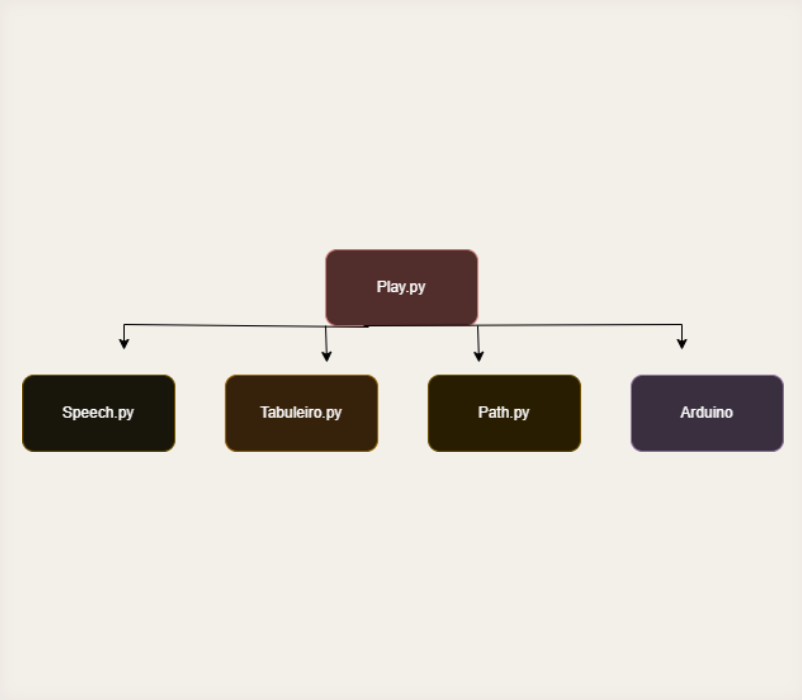
\includegraphics[width=0.7\textwidth]{imagens/esquematizacao_software.png}
    \caption{Esquematização da hierarquia e interação dos módulos de software.}
    \label{fig:arq_software}
\end{figure}

\begin{enumerate}
    \item \textbf{\texttt{speech.py} (Reconhecimento de Voz):} Gerencia a captura de áudio através da biblioteca \texttt{SpeechRecognition} e realiza a transcrição local utilizando o modelo otimizado \texttt{WhisperModel} (\textit{faster-whisper}). O módulo opera como um gerenciador de contexto para manter o microfone calibrado contra ruídos de fundo. Após a transcrição, uma expressão regular filtra a palavra de ativação (\textit{wake word}) ``tabuleiro'' e extrai as coordenadas da jogada em notação padrão SAN ou UCI, convertendo termos como ``rei'', ``dama'' ou ``peão'' para as siglas correspondentes em inglês.
    \item \textbf{\texttt{play.py} (Coordenador Principal):} Funciona como o núcleo lógico da aplicação. Instancia a biblioteca \texttt{chess.Board} para manter o estado oficial do jogo, gerencia a alternância de turnos, inicializa o motor de xadrez Stockfish local via protocolo UCI e coordena as chamadas de movimentação do hardware.
    \item \textbf{\texttt{path.py} (Planejador de Rotas):} Implementa uma subclasse customizada do algoritmo A*, denominada \texttt{TurnPenalizingAStarFinder}. Diferente do A* tradicional, esta variante impõe uma penalidade de custo numérico sempre que há uma mudança na direção do vetor de movimento linear. Isso força o algoritmo a selecionar trajetórias retas, evitando curvas desnecessárias e tornando o movimento mais natural. Adicionalmente, possui uma função de otimização que elimina nós colineares, transmitindo ao hardware apenas os vértices de mudança de curso.
    \item \textbf{\texttt{tabuleiro.py} (\texttt{BoardManager}):} Modela matematicamente a área física do tabuleiro expandido em uma matriz $37 \times 37$ representada via \texttt{pandas.DataFrame}. Essa grade estendida inclui as 64 casas centrais de jogo, a delimitação virtual das peças e duas colunas de descarte lateral (\texttt{E0} para brancas capturadas e \texttt{D2} para pretas capturadas). Esse mapeamento é crucial para evitar colisões físicas durante a passagem das peças entre as casas e para gerenciar a remoção de peças do tabuleiro.
    \item \textbf{\texttt{Arduino.cpp} (Firmware):} Desenvolvido para o microcontrolador ATmega328P. Controla os drivers A4988 utilizando a biblioteca \texttt{FastAccelStepper}, que gera pulsos baseados em interrupções de timer de hardware, garantindo aceleração suave. Implementa uma máquina de estados serial acionada por caracteres de comando específicos (\texttt{T} para trajetórias, \texttt{P} para modo jogo, \texttt{C} para calibração, \texttt{H} para \textit{home} e \texttt{D} para depuração).
\end{enumerate}

\begin{figure}[htpb]
    \centering
    \begin{subfigure}[b]{0.45\textwidth}
        \centering
        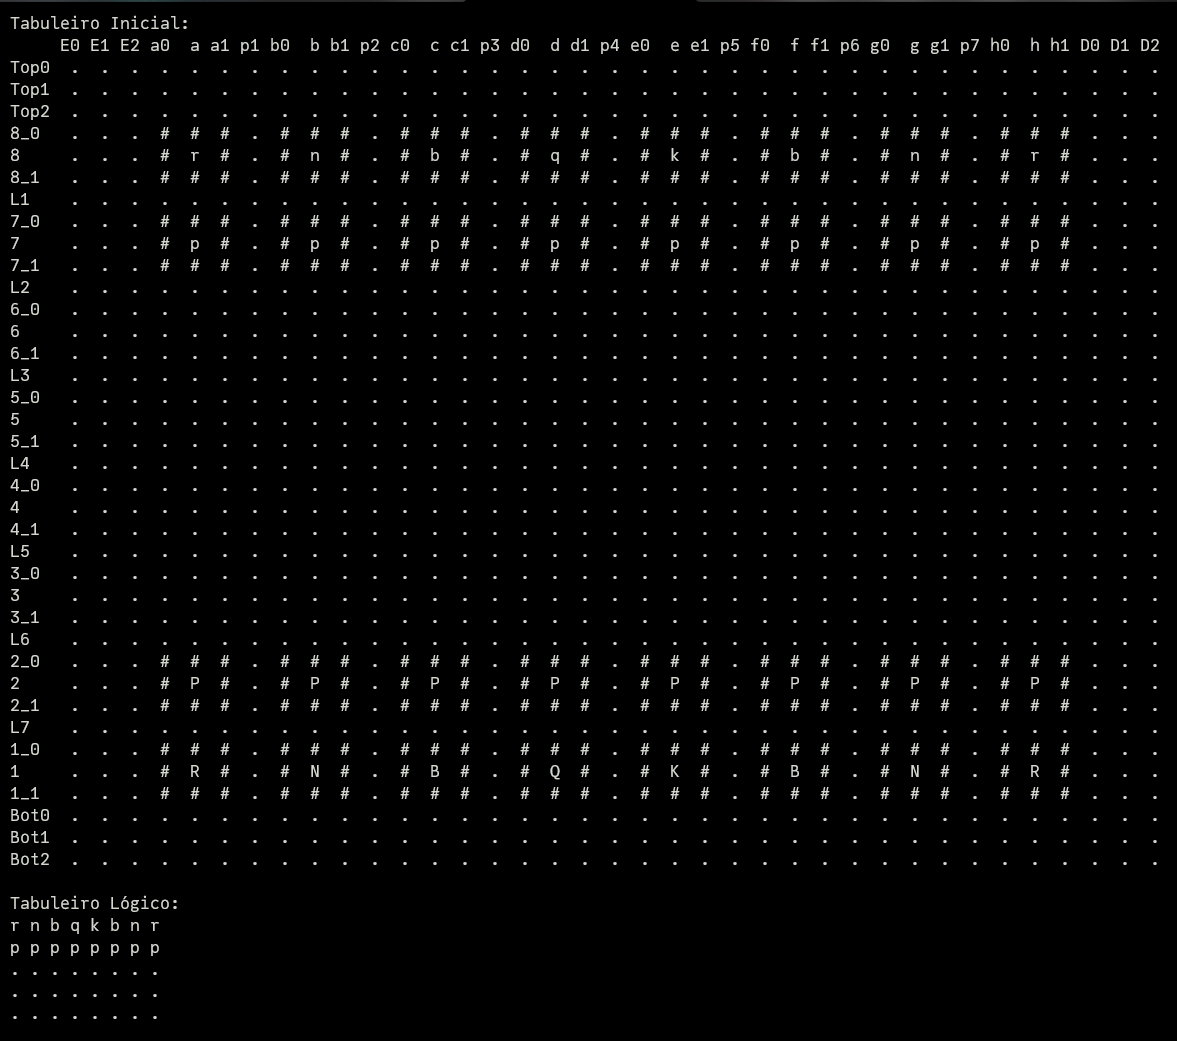
\includegraphics[width=\textwidth]{imagens/tabuleiro_matriz.png}
        \caption{Matriz gerada pelo \texttt{tabuleiro.py}.}
    \end{subfigure}
    \hfill
    \begin{subfigure}[b]{0.45\textwidth}
        \centering
        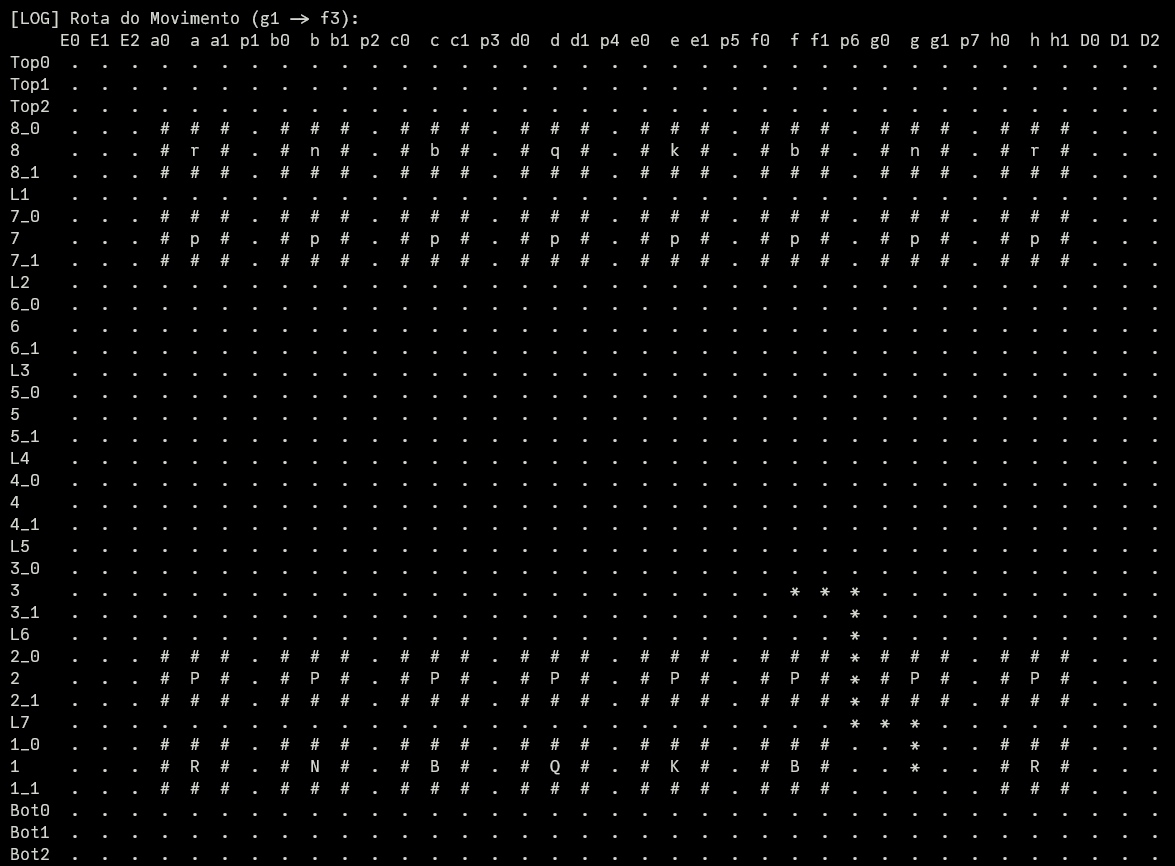
\includegraphics[width=\textwidth]{imagens/rota.png}
        \caption{Rota calculada pelo algoritmo A*.}
    \end{subfigure}
    \caption{Representações internas de estado e planejamento de rota visíveis no terminal.}
    \label{fig:matrizes}
\end{figure}

O planejamento de trajetória utiliza um protocolo síncrono por passos para transmissão serial a 115200 baud e envio das coordenadas em partes, garantindo que o Arduino nunca sofra estouro de \textit{buffer}:
\begin{verbatim}
PC  ---> Envia "T{n}" (Avisa trajetória com n pontos)
MCU ---> Responde "READY_FOR_POINTS" após acordar os drivers
PC  ---> Envia "X_0 Y_0" (Primeira coordenada de curva)
MCU ---> Executa movimento linear, sobe o servo e responde "POINT_OK" 
...
PC  ---> Envia "X_n Y_n" (Último ponto)
MCU ---> Abaixa o servo, desativa drivers e responde "TRAJETORIA OK"
\end{verbatim}

\section{Desenvolvimento do Circuito Eletrônico}
A eletrônica do projeto exigiu modificações em relação à esquematização inicial para implementar novas funcionalidades, como o \textit{microstepping} para o controle fino e suave dos motores e um LED para indicar que a fonte de alimentação está corretamente conectada. O diagrama elétrico inicial e o final estão representados na Figura \ref{fig:circuitos_esquemas}.

\begin{figure}[htpb]
    \centering
    \begin{subfigure}[b]{0.45\textwidth}
        \centering
        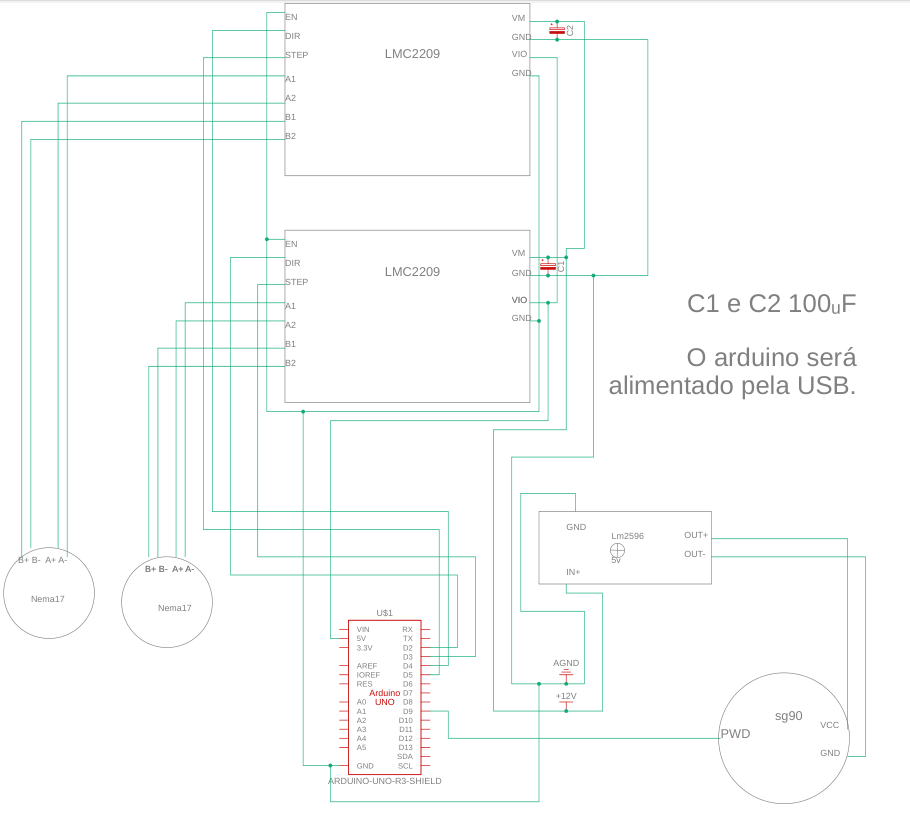
\includegraphics[width=\textwidth]{imagens/circuito1.png}
        \caption{Primeira esquematização do circuito.}
        \label{fig:circuito_inicial}
    \end{subfigure}
    \hfill
    \begin{subfigure}[b]{0.45\textwidth}
        \centering
        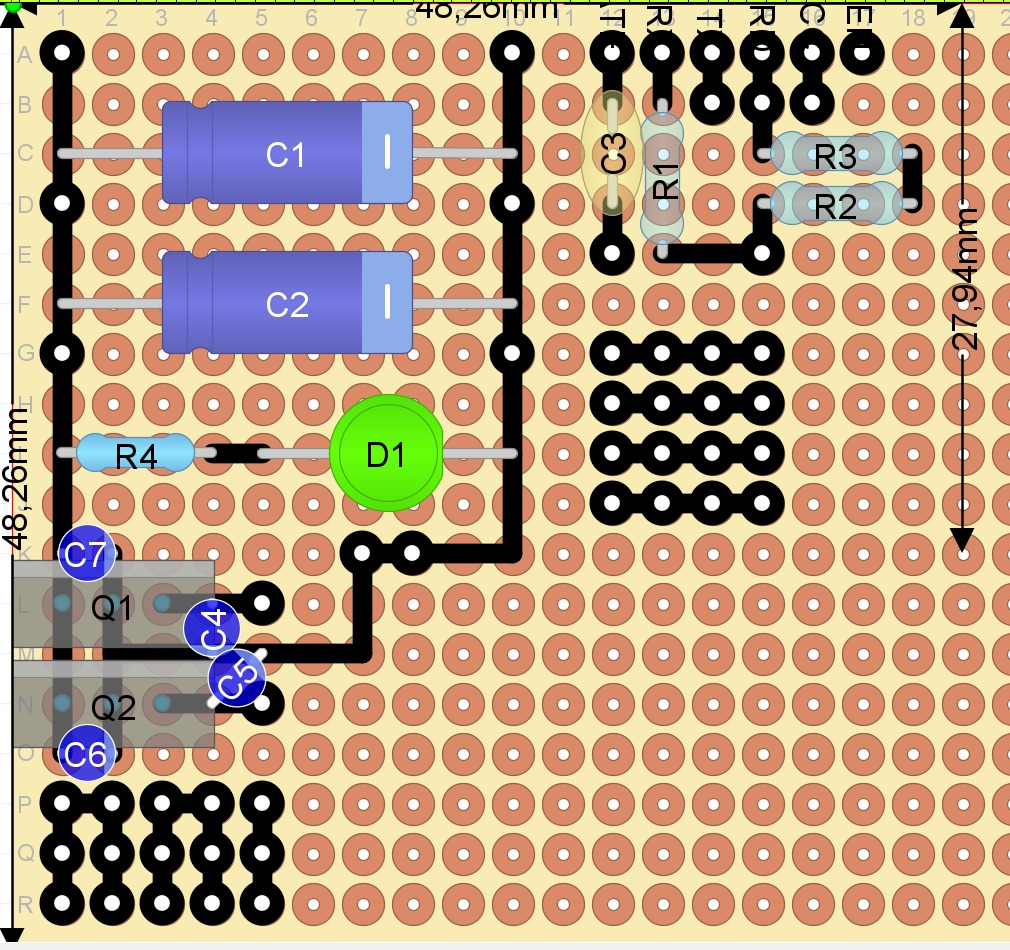
\includegraphics[width=\textwidth]{imagens/circuito3.jpeg}
        \caption{Esquematização final atualizada com novos módulos.}
    \end{subfigure}
    \caption{Evolução do diagrama eletrônico do projeto.}
    \label{fig:circuitos_esquemas}
\end{figure}

\subsection{Problemas Identificados e Soluções Adotadas}
\begin{itemize}
    \item \textbf{Uso dos drivers A4988:} As tentativas iniciais de controle dos motores foram frustrantes devido ao mau funcionamento de três dos cinco drivers disponíveis. Por serem componentes sensíveis, exigem o uso de capacitores de desacoplamento robustos e cuidados no manuseio dos \textit{jumpers} para evitar descargas eletrostáticas no \textit{chip}. A identificação do mau funcionamento foi possível através da verificação da saída (\textit{output}) para os motores no osciloscópio, que exibia um sinal contínuo em vez de pulsos. Outro \textit{driver} foi danificado devido à troca de \textit{jumpers} com o circuito ainda energizado. A solução consistiu na substituição dos componentes danificados e na implementação de um LED para indicação visual do estado de alimentação.
    \item \textbf{Superaquecimento por Corrente de Holding:} Inicialmente, os motores NEMA 17 permaneciam energizados continuamente. A corrente de manutenção estática (\textit{holding current}) gerava aquecimento desnecessário nos motores. A solução foi mapear o pino \texttt{ENABLE} de ambos os drivers ao pino digital \texttt{PIN\_SLEEP} do Arduino. O firmware agora coloca os drivers em modo de baixo consumo imediatamente após o término de qualquer movimento, reativando-os apenas quando uma nova trajetória é recebida. 
    \item \textbf{Instabilidade e Ruído no Servo Motor:} O servo motor utilizado no atuador vertical sofria com picos de corrente durante o funcionamento, o que derrubava a tensão de 5V do barramento do Arduino, causando \textit{resets} intermitentes do processador. Para solucionar isso, isolou-se a alimentação do servo utilizando um regulador linear de tensão \texttt{LM7805} conectado diretamente à fonte principal de 12V. Foram inseridos dois capacitores de desacoplamento de $10\,\mu\text{F}$ (um na entrada e outro na saída do regulador) para filtrar transientes e ruídos na linha de sinal.
    \item \textbf{Falhas de Comunicação Sem Fio:} A tentativa inicial de utilizar um módulo Bluetooth HC-05 para comunicação com o computador rodando o Windows 11 apresentou instabilidades críticas de pareamento e perdas de pacotes de dados no protocolo serial. Como solução definitiva, optou-se pela conexão física estável via cabo USB nativo, operando a uma taxa estável de 115200 baud. Os pinos que haviam sido reservados no circuito soldado para o módulo Bluetooth foram redirecionados para o barramento de controle estático (\texttt{Sleep} e \texttt{Reset}) dos drivers de passo. Manter ambos os pinos em nível lógico alto (\texttt{HIGH}) garante que os drivers permaneçam ativos e não entrem em modo de economia inadvertidamente, evitando travamentos inesperados.
\end{itemize}

\begin{figure}[htpb]
    \centering
    \begin{subfigure}[b]{0.45\textwidth}
        \centering
        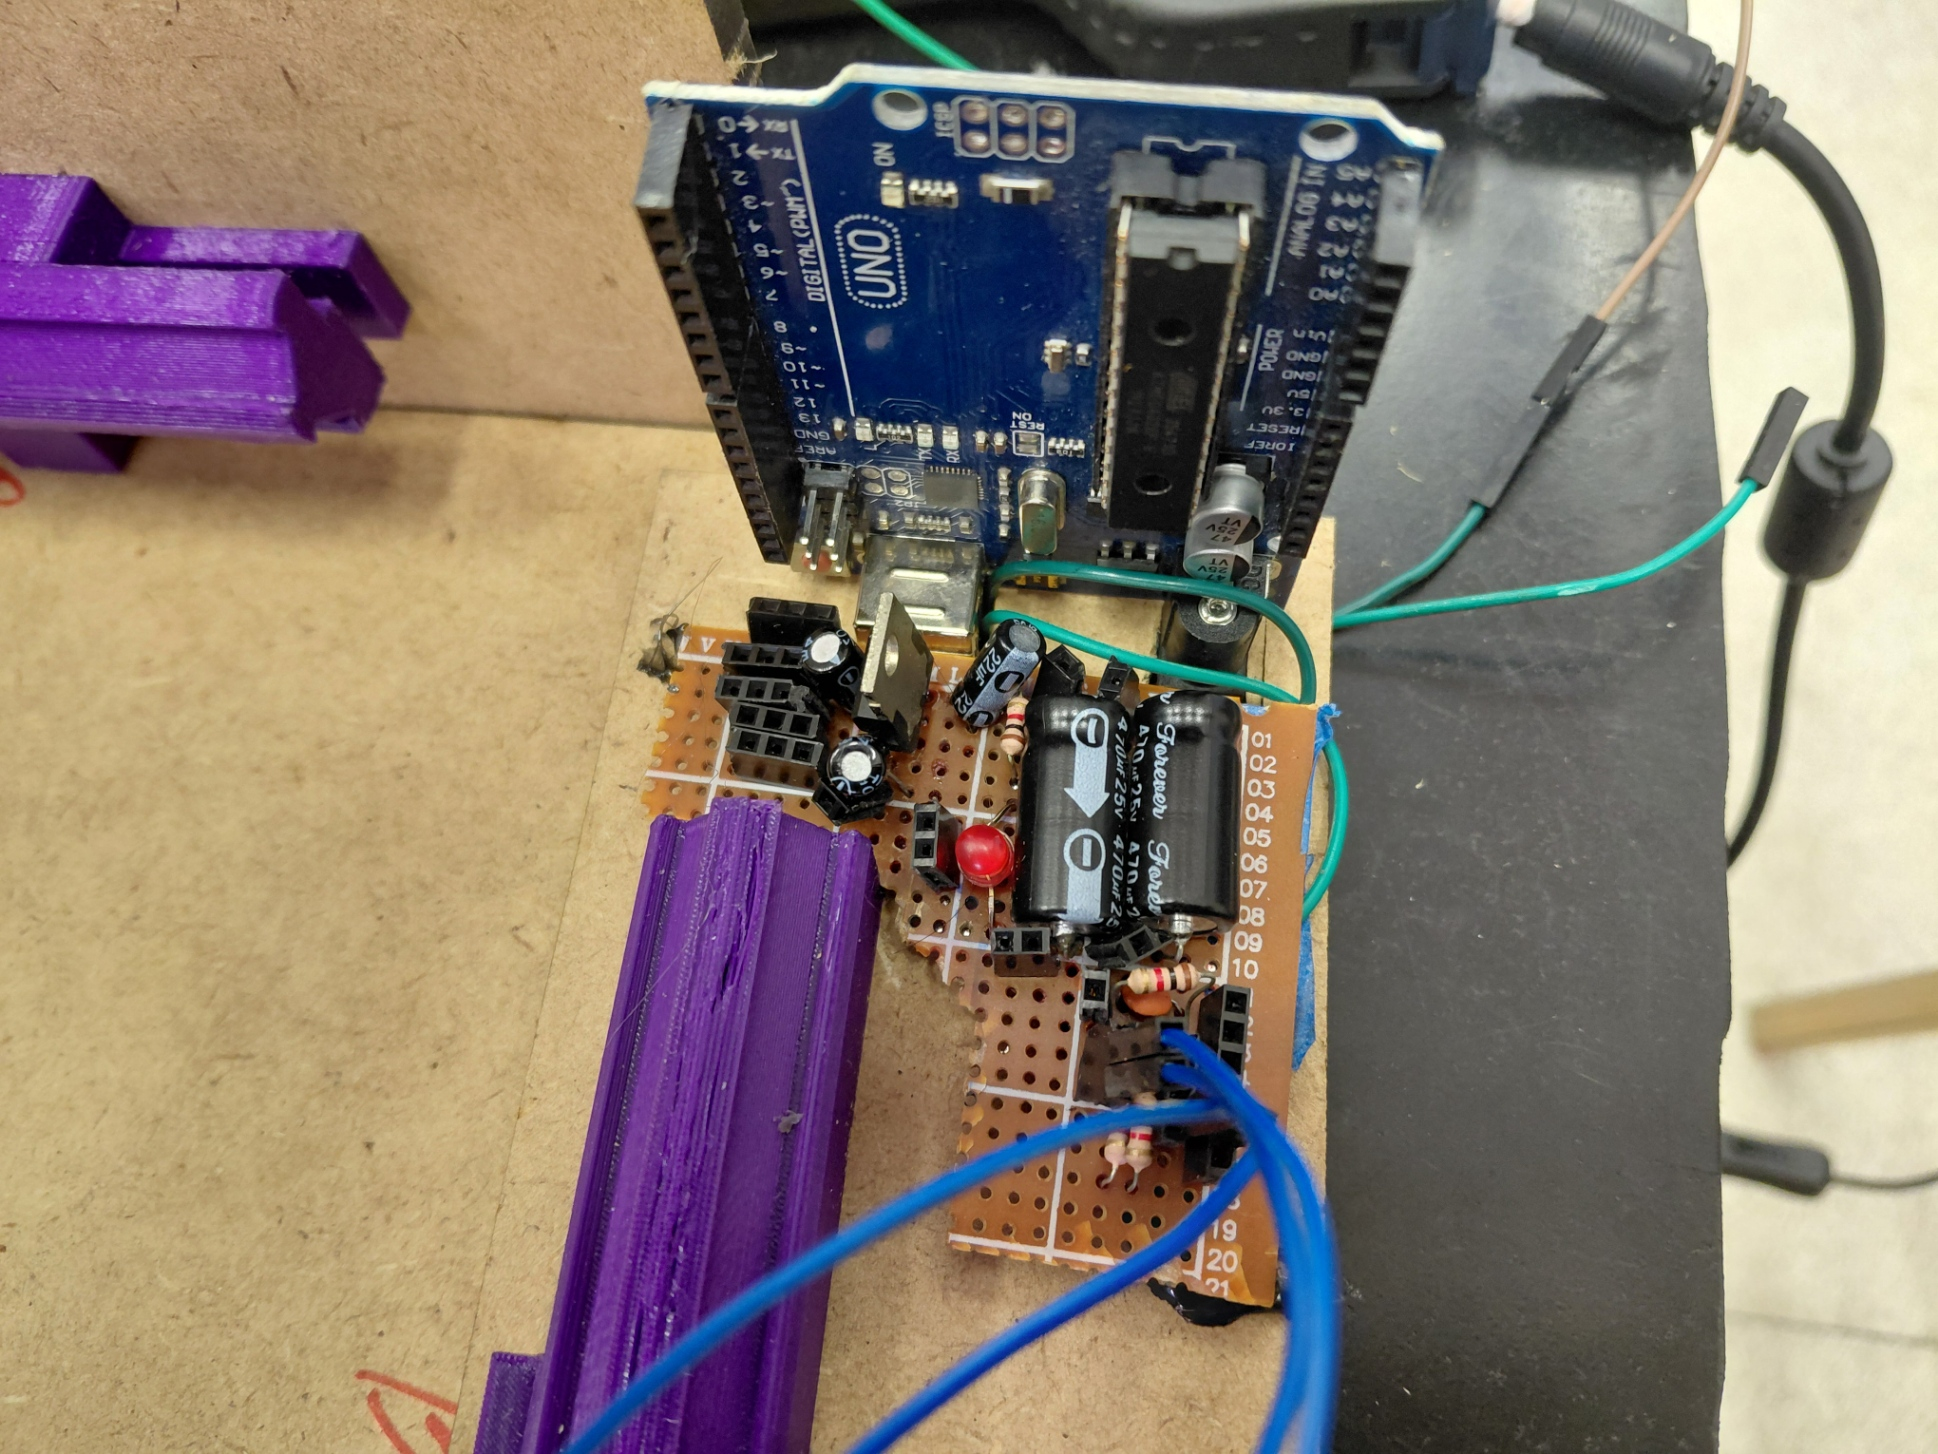
\includegraphics[width=\textwidth]{imagens/circuito2.jpg}
        \caption{Placa de circuito final soldada.}
    \end{subfigure}
    \hfill
    \begin{subfigure}[b]{0.45\textwidth}
        \centering
        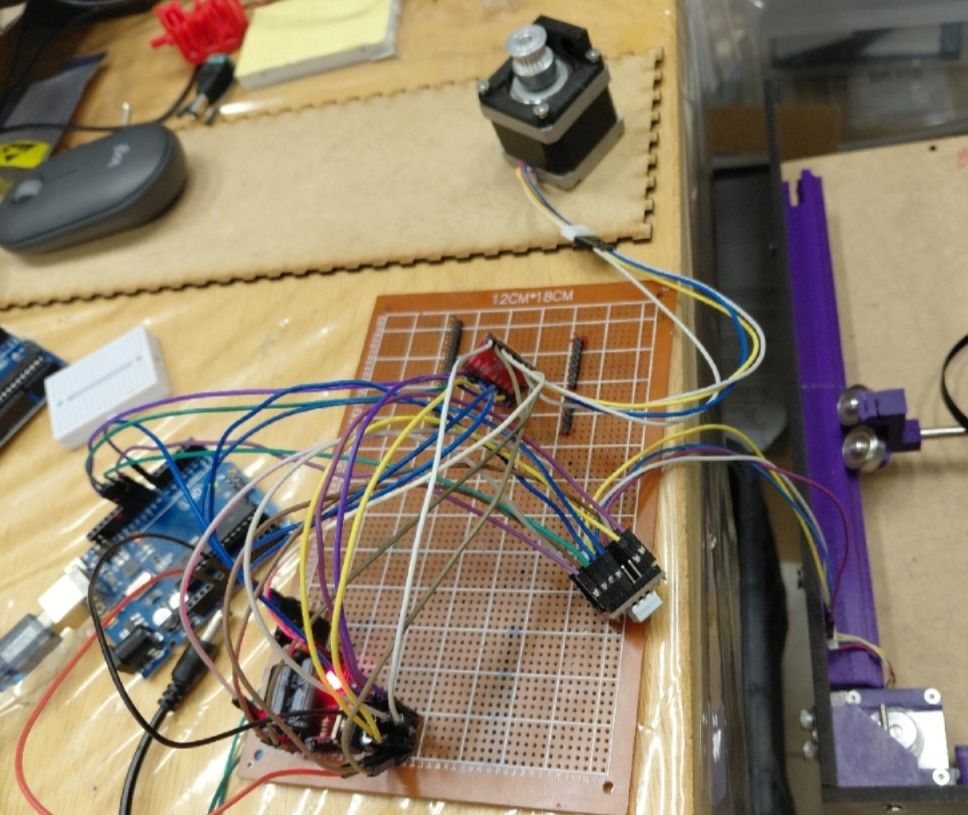
\includegraphics[width=\textwidth]{imagens/circuito1.jpg}
        \caption{Teste do circuito em bancada com drivers e motores.}
    \end{subfigure}
    \caption{Implementação física do circuito eletrônico.}
    \label{fig:circuito_fisico}
\end{figure}

\section{Implementação Mecânica e Estrutural}
A construção física do sistema representou o maior desafio de engenharia do projeto, exigindo sucessivos ciclos de testes, erros e soluções de contorno devido à ausência de componentes industriais padrão, como eixos lineares retificados de aço.

\subsection{Configuração de Eixos e Dinâmica}
Optou-se por posicionar os motores NEMA 17 de forma fixa e diagonalmente oposta nas quinas da estrutura (canto inferior direito e superior esquerdo). Suas correias sincronizadoras estendem-se até polias localizadas no canto inferior esquerdo. Cada motor atua independentemente sobre um eixo cartesiano. Embora mecanicamente simples e eficiente para reduzir a inércia móvel (mantendo o centro de gravidade estático nos motores), essa configuração exige um alinhamento perfeito; qualquer assimetria nas forças gera um torque no carrinho móvel, resultando em travamento instantâneo por fricção. O arranjo pode ser visto na Figura \ref{fig:motores}.

\begin{figure}[htpb]
    \centering
    \begin{subfigure}[b]{0.32\textwidth}
        \centering
        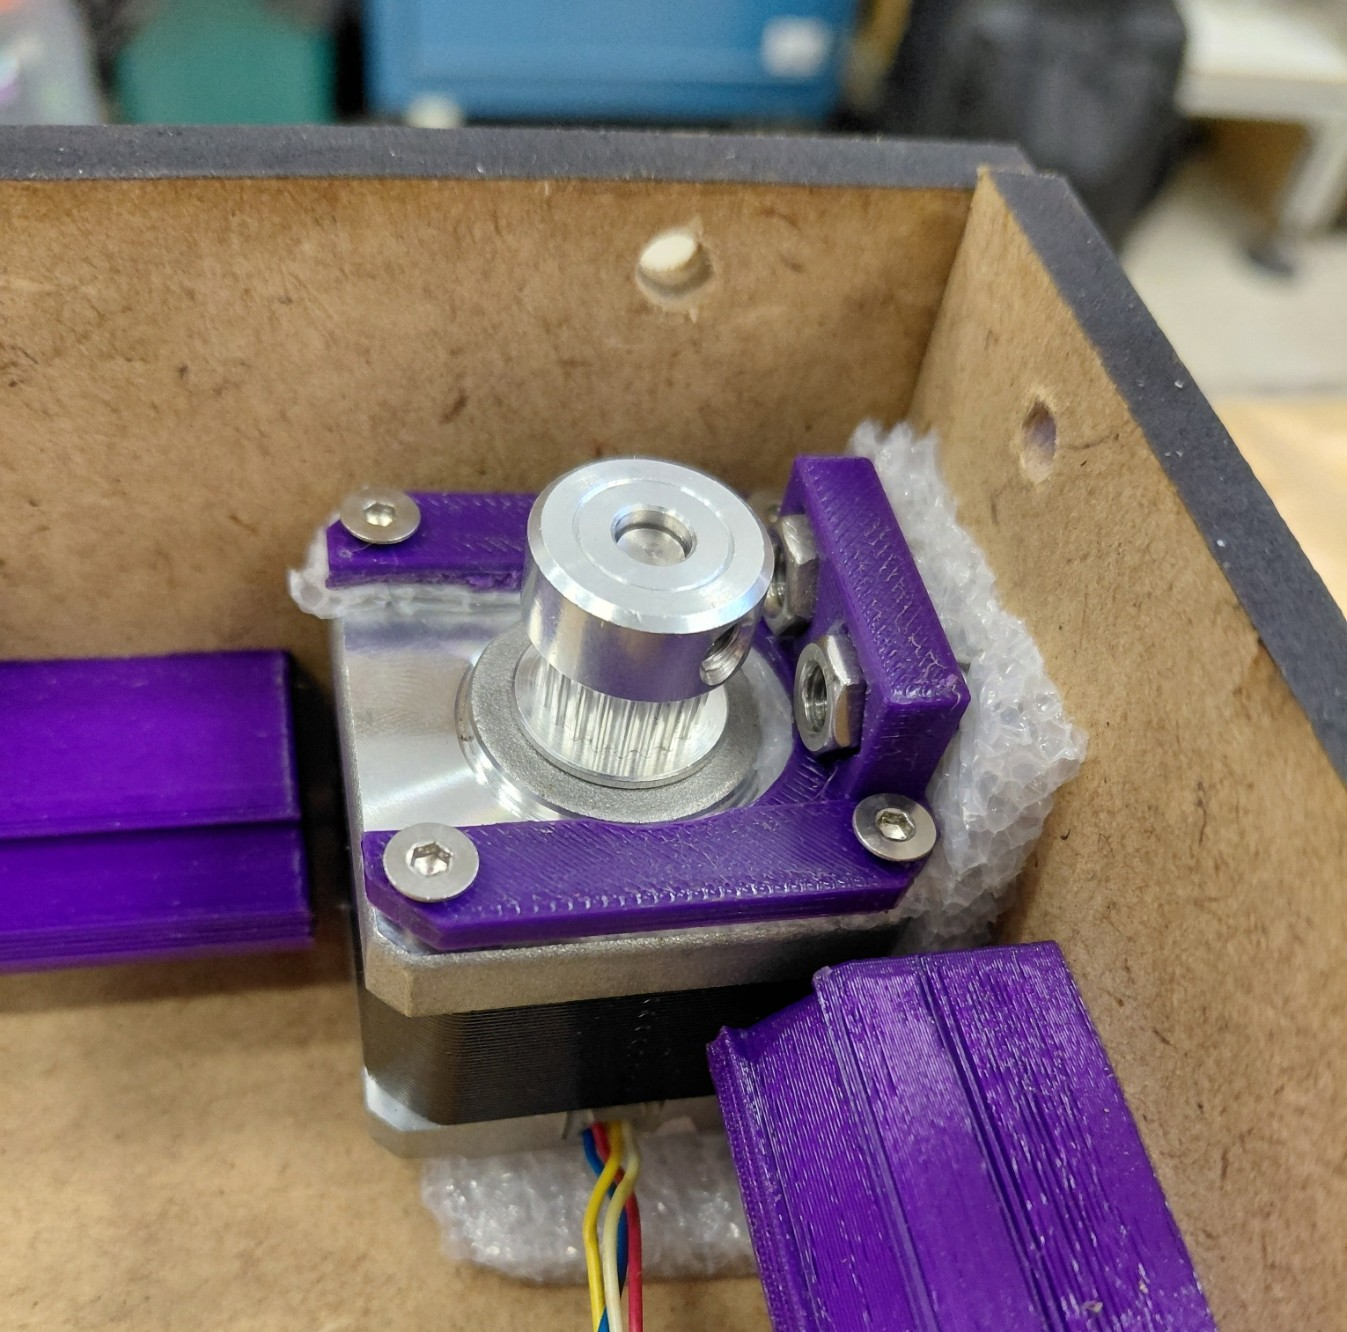
\includegraphics[width=\textwidth]{imagens/motor1.jpg}
        \caption{Motor superior esquerdo.}
    \end{subfigure}
    \hfill
    \begin{subfigure}[b]{0.32\textwidth}
        \centering
        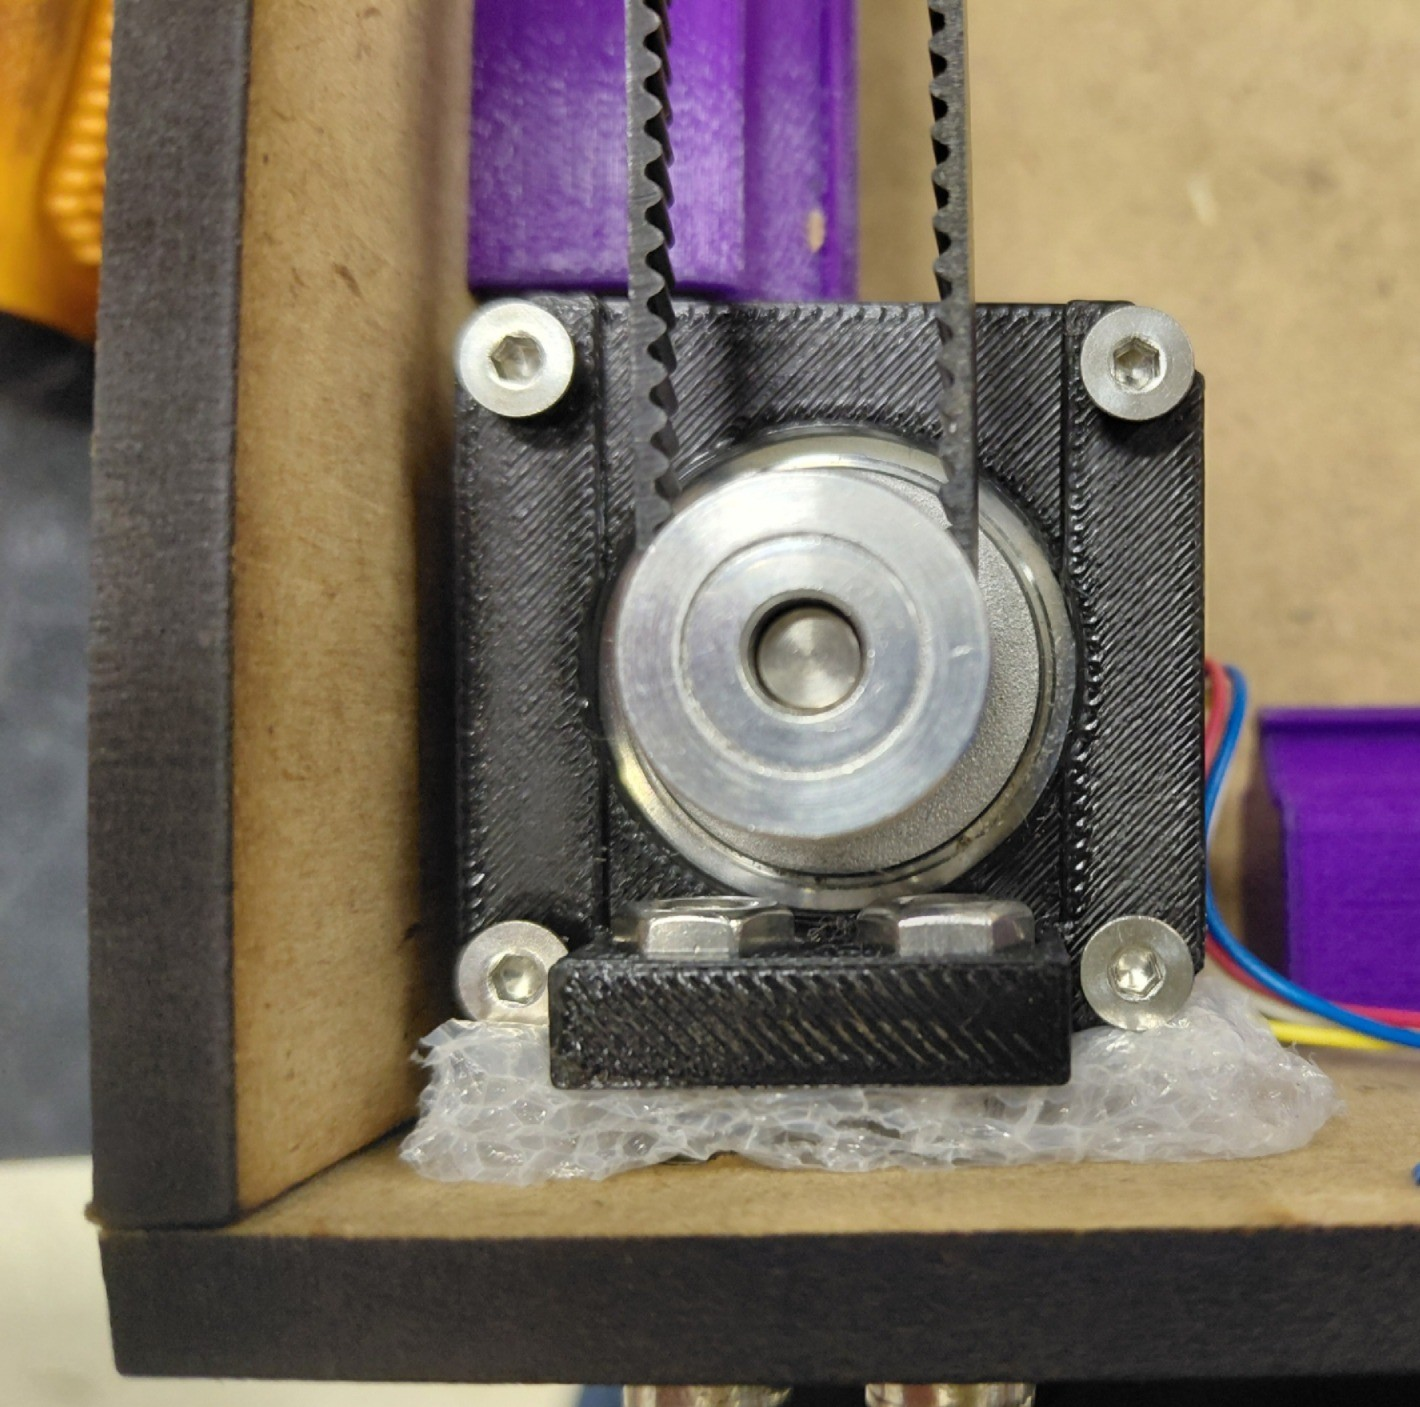
\includegraphics[width=\textwidth]{imagens/motor2.jpg}
        \caption{Motor inferior direito.}
    \end{subfigure}
    \hfill
    \begin{subfigure}[b]{0.32\textwidth}
        \centering
        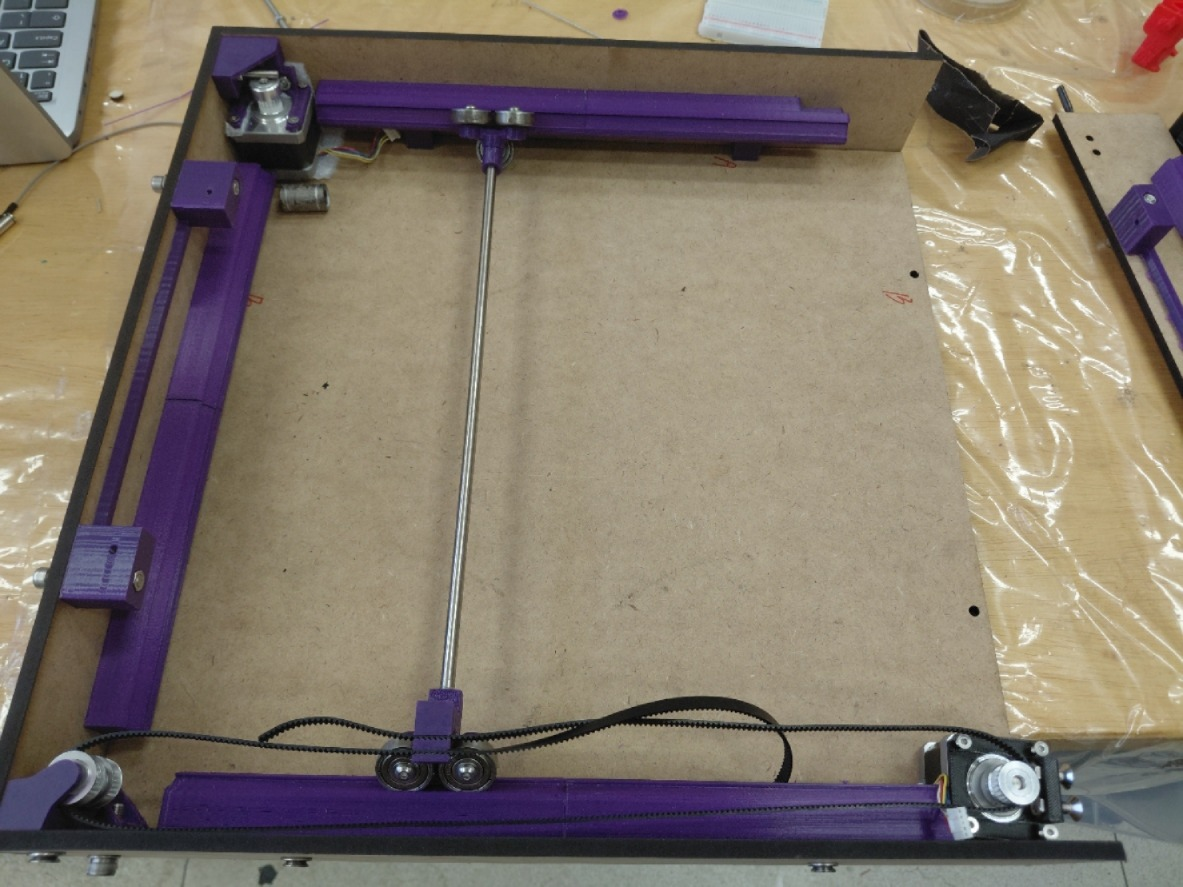
\includegraphics[width=\textwidth]{imagens/motores.jpg}
        \caption{Visão geral do tracionamento.}
    \end{subfigure}
    \caption{Posicionamento dos motores NEMA 17 e roteamento das correias.}
    \label{fig:motores}
\end{figure}

\subsection{Fabricação dos Trilhos em V e Carrinhos}
Na ausência de guias lineares metálicas, projetou-se trilhos planos com inclinação de 45° e carrinhos sob medida para impressão 3D, utilizando rolamentos rígidos de esferas modelo 608zz como roletes de contato. Esse modelo foi inspirado em trilhos comerciais com formato \textit{V-slot} (Figura \ref{fig:mecanica_linear}).

\begin{figure}[htpb]
    \centering
    \begin{subfigure}[b]{0.32\textwidth}
        \centering
        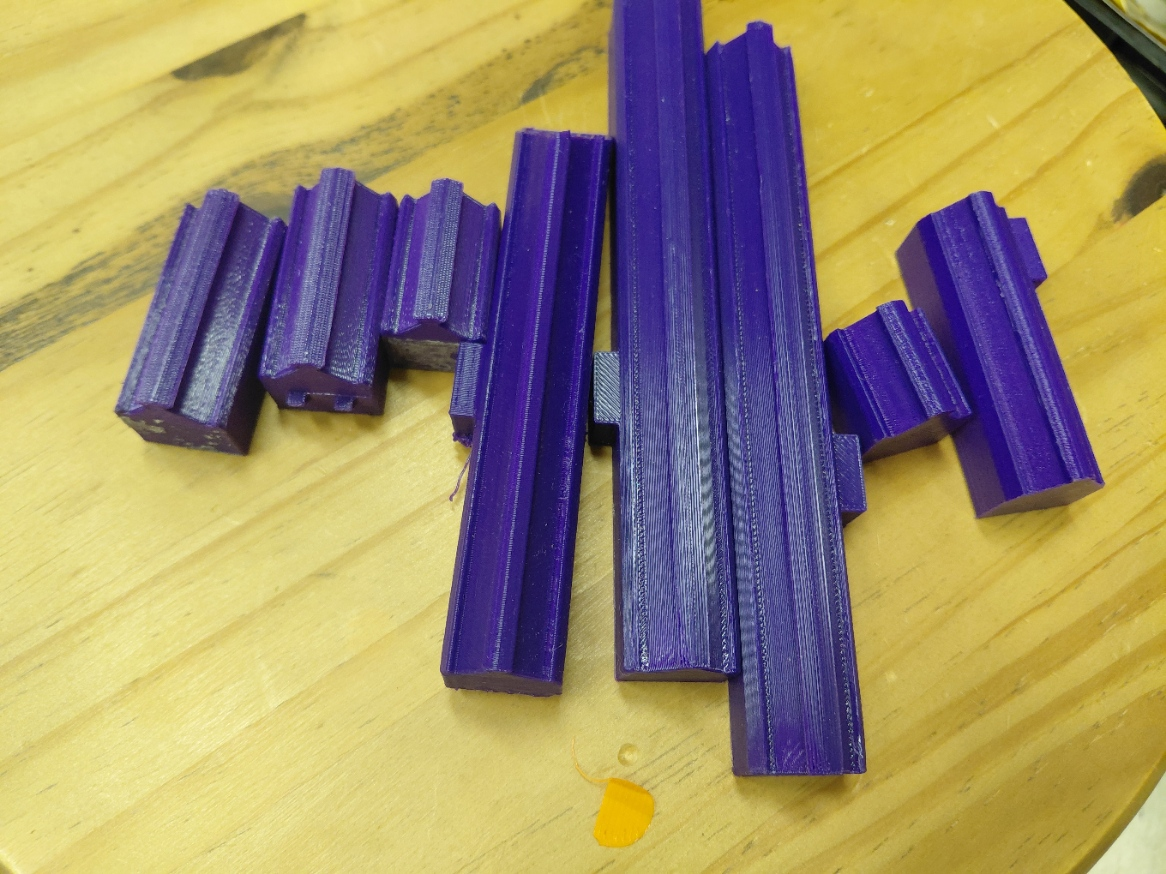
\includegraphics[width=\textwidth]{imagens/testestrilhos.jpg}
        \caption{Testes de impressão.}
    \end{subfigure}
    \hfill
    \begin{subfigure}[b]{0.32\textwidth}
        \centering
        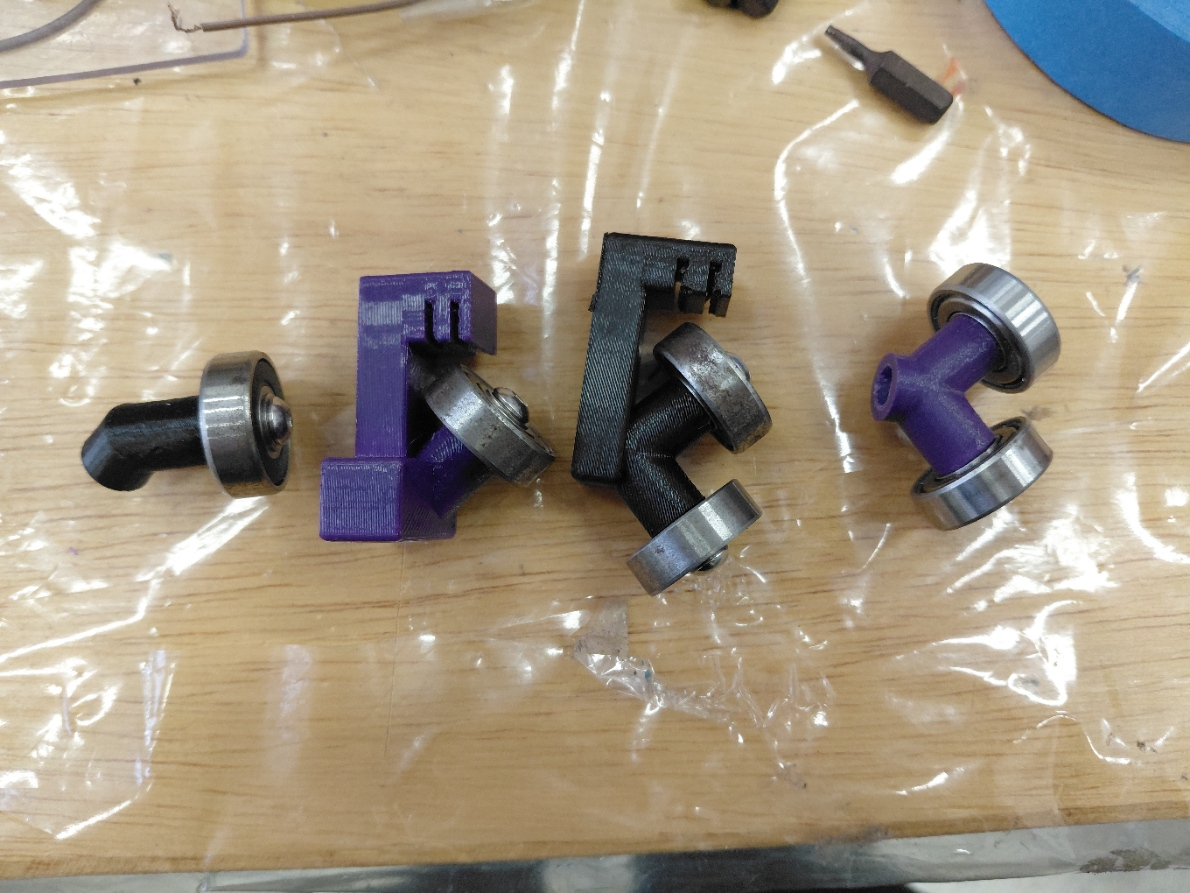
\includegraphics[width=\textwidth]{imagens/carrinhos.jpg}
        \caption{Carrinhos deslizantes.}
    \end{subfigure}
    \hfill
    \begin{subfigure}[b]{0.32\textwidth}
        \centering
        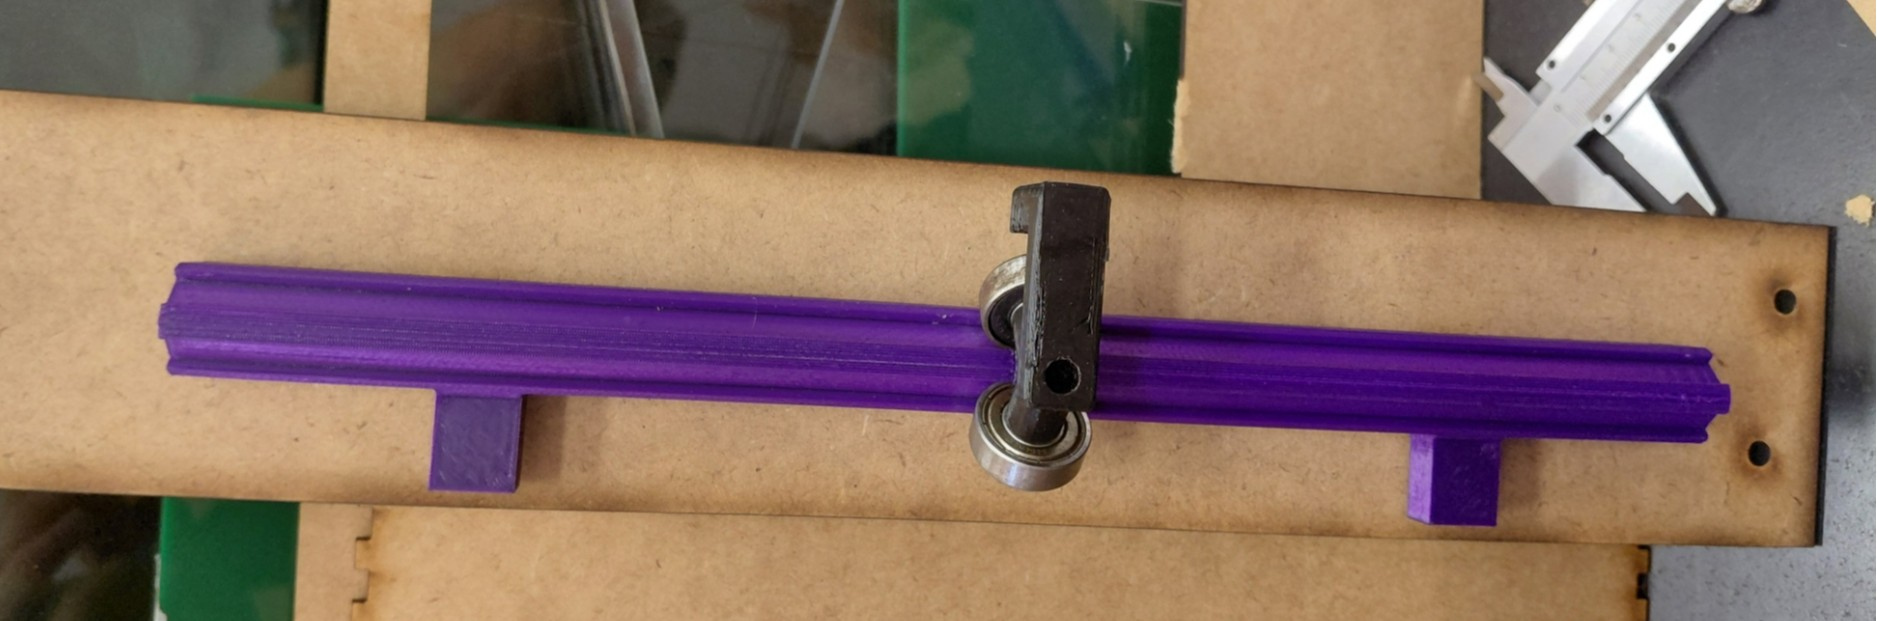
\includegraphics[width=\textwidth]{imagens/carrinho_trilho.jpg}
        \caption{Encaixe no trilho.}
    \end{subfigure}
    
    \vspace{1em}
    
    \begin{subfigure}[b]{0.32\textwidth}
        \centering
        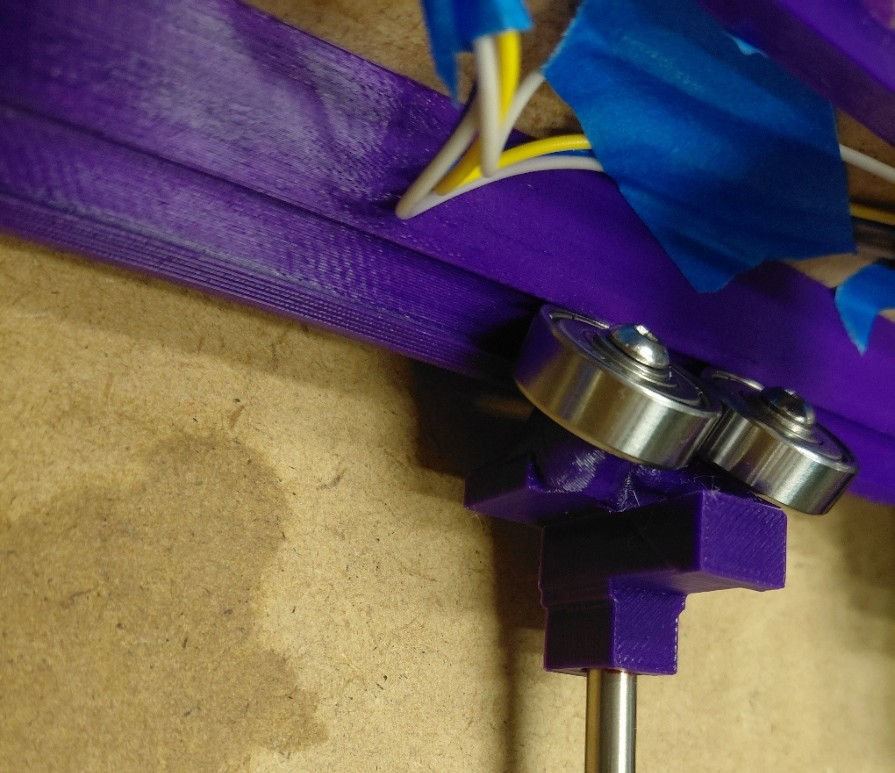
\includegraphics[width=\textwidth]{imagens/novocarrinho1.jpg}
        \caption{Redesign do carrinho.}
        \label{fig:novo_carrinho}
    \end{subfigure}
    \hfill
    \begin{subfigure}[b]{0.32\textwidth}
        \centering
        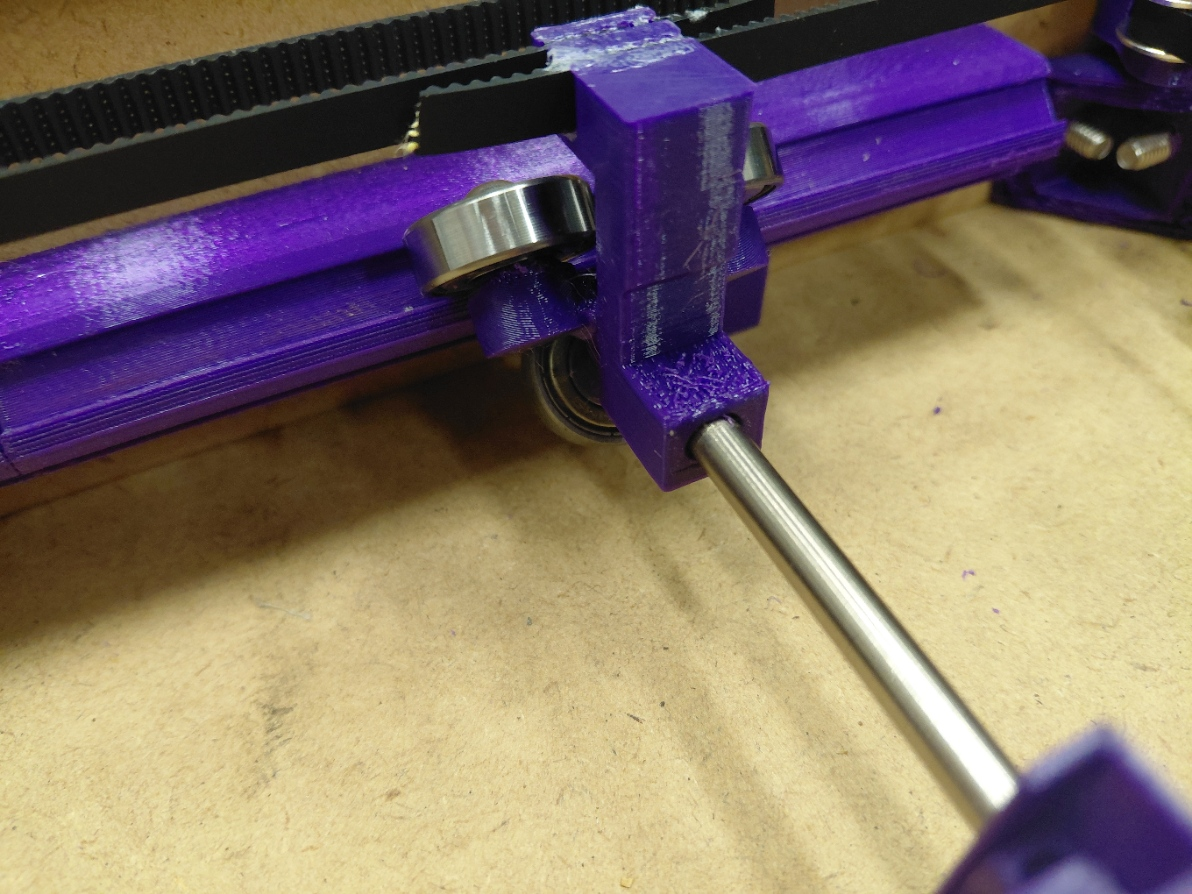
\includegraphics[width=\textwidth]{imagens/novocarrinho2.jpg}
        \caption{Redesign em uso.}
    \end{subfigure}
    \hfill
    \begin{subfigure}[b]{0.32\textwidth}
        \centering
        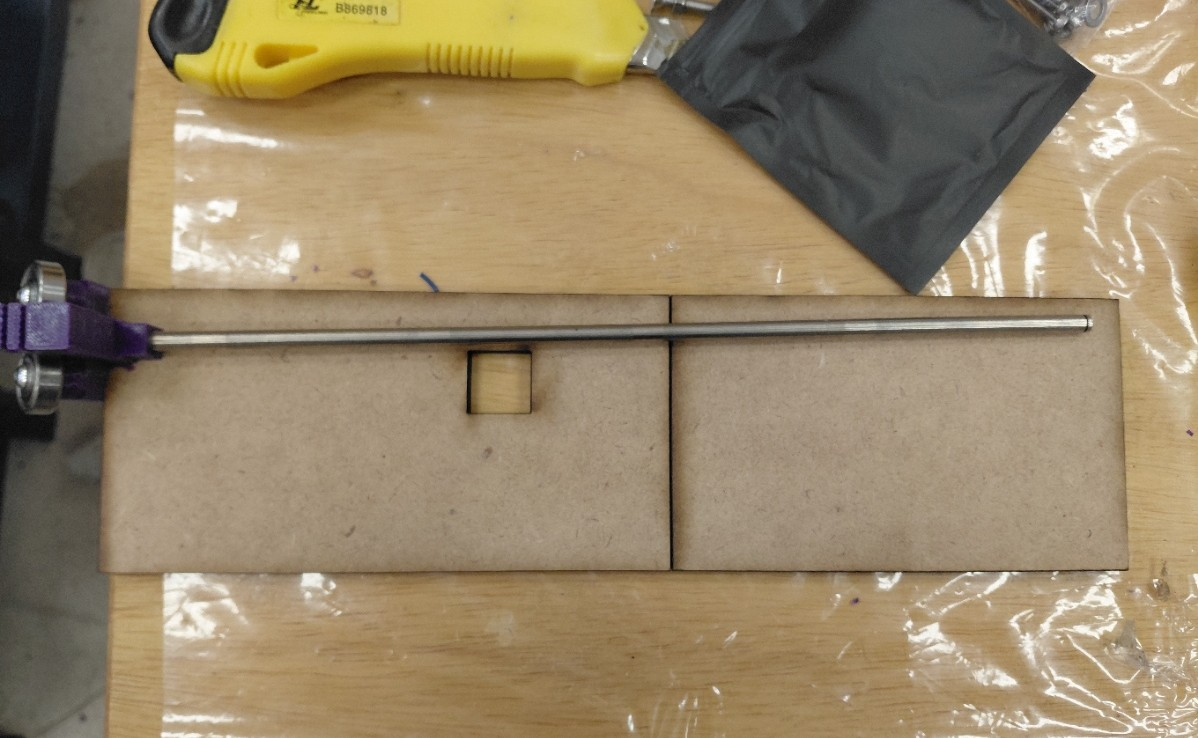
\includegraphics[width=\textwidth]{imagens/encaixetorto.jpg}
        \caption{Desvio ao encaixar a barra.}
        \label{fig:eixo_flutuante}
    \end{subfigure}
    \caption{Desenvolvimento iterativo do sistema mecânico linear, carrinhos e ajuste de eixo.}
    \label{fig:mecanica_linear}
\end{figure}

\begin{itemize}
    \item \textbf{Problema de Instabilidade Rotacional:} A primeira iteração contava com dois rolamentos no braço superior do carrinho e apenas um no braço inferior. Sob ação da tração da correia, o conjunto sofria deflexão angular e girava facilmente sobre o trilho, travando o sistema. A solução foi redesenhar o carrinho adicionando um segundo rolamento de estabilização na face superior, distribuindo o torque uniformemente (Figura \ref{fig:novo_carrinho}).
    \item \textbf{Retificação das Barras:} Intercorrências na montagem demonstraram que as barras de $6\,\text{mm}$ acopladas ao carrinho ficavam levemente desalinhadas devido a pequenas imperfeições de impressão dos carrinhos. A solução consistiu na aplicação de enxertos estruturais até atingir um alinhamento tolerável (Figura \ref{fig:eixo_flutuante})..
    \item \textbf{Descontinuidades de Impressão:} O comprimento total do tabuleiro excedia o volume útil de impressão da máquina disponível. Os trilhos precisaram ser seccionados em duas partes e colados manualmente. Apesar do lixamento, a pequena descontinuidade na junção das partes coladas atuava como um obstáculo geométrico onde os rolamentos colidiam e travavam.
    \item \textbf{Imprecisão Dimensional das Paredes:} Pequenas variações milimétricas no paralelismo das paredes de MDF empurravam os carrinhos para dentro ou para fora. Como os carrinhos eram rigidamente acoplados à barra transversal de ferro, qualquer aproximação das paredes causava compressão excessiva nos trilhos, paralisando os motores.
    \item \textbf{Solução Implementada (Eixo Flutuante):} Para resolver o travamento por variação de largura, eliminou-se a restrição rígida de uma das extremidades da barra de ferro transversal. Ela passou a operar como um ``eixo flutuante'', livre para deslizar para dentro ou para fora do encaixe do carrinho conforme a distância entre as paredes variava. Essa folga geométrica sanou os travamentos por compressão, porém introduziu uma perda de rigidez estrutural: a barra passou a flexionar sob torção, gerando um novo vetor de torque que limitou a movimentação nas proximidades dos carrinhos dotados de eixo flutuante. 
\end{itemize}

\subsection{Atuador Vertical de Altura do Ímã}
Para acoplar e desacoplar magneticamente as peças dispostas na superfície superior do tabuleiro, implementou-se um mecanismo de transformação de movimento rotacional em linear baseado em pinhão e cremalheira acionado por um servo motor (Figura \ref{fig:servo}). Por questões de montagem física, a lógica angular atuou de forma invertida: o pulso equivalente a 180° causava o recuo vertical da cremalheira e o de 40° realizava a suspensão mecânica do conjunto, aproximando o ímã de neodímio da tampa de acrílico. Quando o comando serial finaliza, o acoplamento magnético é rompido de forma controlada para que o carrinho possa se deslocar livremente sem arrastar peças indesejadas. Esta solução mostrou-se compacta, leve e de alta confiabilidade.

\begin{figure}[htpb]
    \centering
    \begin{subfigure}[b]{0.32\textwidth}
        \centering
        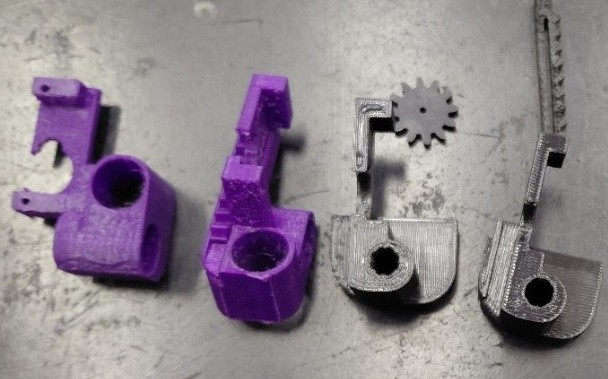
\includegraphics[width=\textwidth]{imagens/testescarrinhos.jpg}
        \caption{Impressões de teste.}
    \end{subfigure}
    \hfill
    \begin{subfigure}[b]{0.32\textwidth}
        \centering
        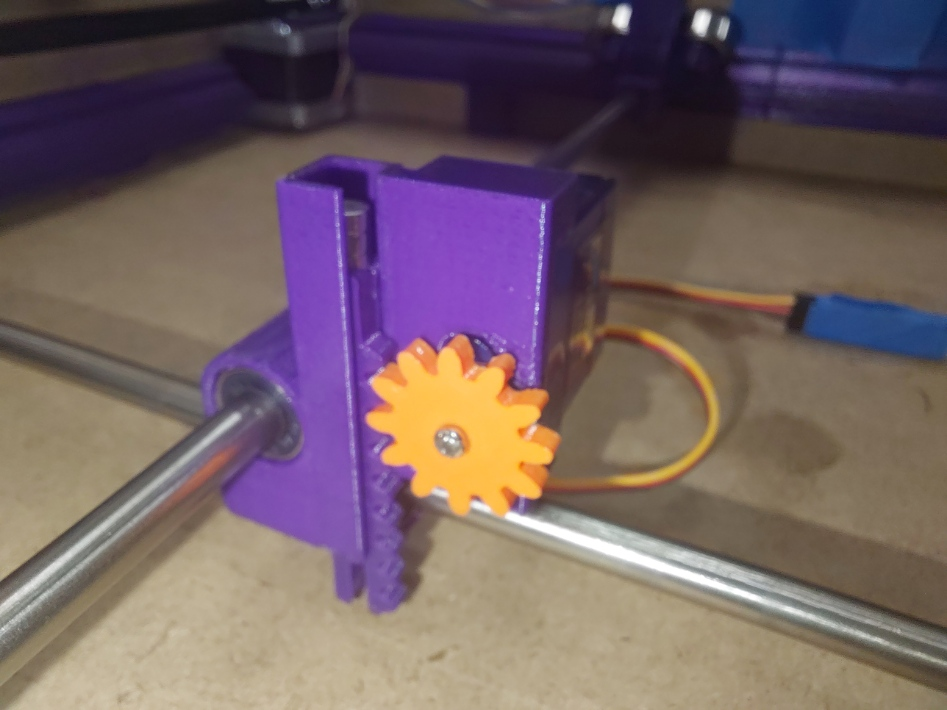
\includegraphics[width=\textwidth]{imagens/carrinhoservo2.jpg}
        \caption{Cremalheira retraída.}
    \end{subfigure}
    \hfill
    \begin{subfigure}[b]{0.32\textwidth}
        \centering
        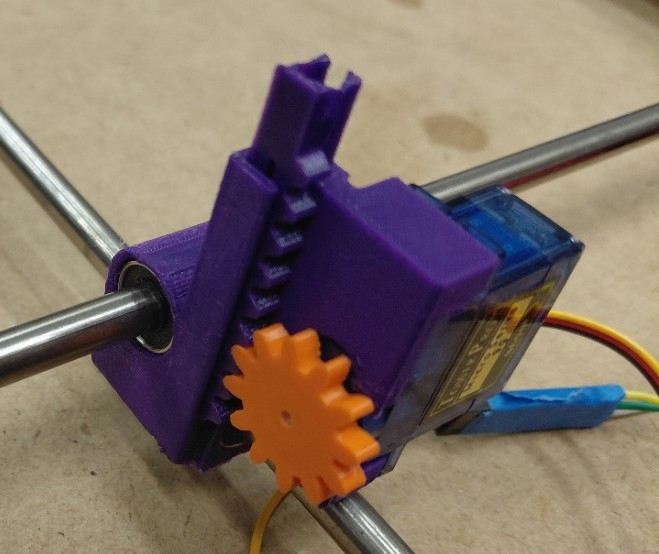
\includegraphics[width=\textwidth]{imagens/carrinhoservo.jpg}
        \caption{Cremalheira esticada.}
    \end{subfigure}
    \caption{Atuador vertical magnético com sistema de pinhão e cremalheira acionado por servo.}
    \label{fig:servo}
\end{figure}

\subsection{Estrutura de MDF e Tolerâncias de Montagem}
A carcaça externa foi cortada em MDF de 6mm utilizando uma cortadora a laser (Figura \ref{fig:laser_falhas}). Durante o processo, a máquina apresentou falhas de oscilação intermitente de potência, necessitando de múltiplas passagens lentas sobre o mesmo vetor. Como efeito colateral, a largura do corte excedeu o planejado (fenômeno de \textit{kerf}), queimando as bordas deixando o encaixe frouxo. A perda de rigidez resultante impediria o tensionamento correto das correias e a fixação dos motores. A estabilidade estrutural foi restabelecida através da instalação manual de duas cantoneiras impressas nos cantos críticos.

\begin{figure}[htpb]
    \centering
    \begin{subfigure}[b]{0.45\textwidth}
        \centering
        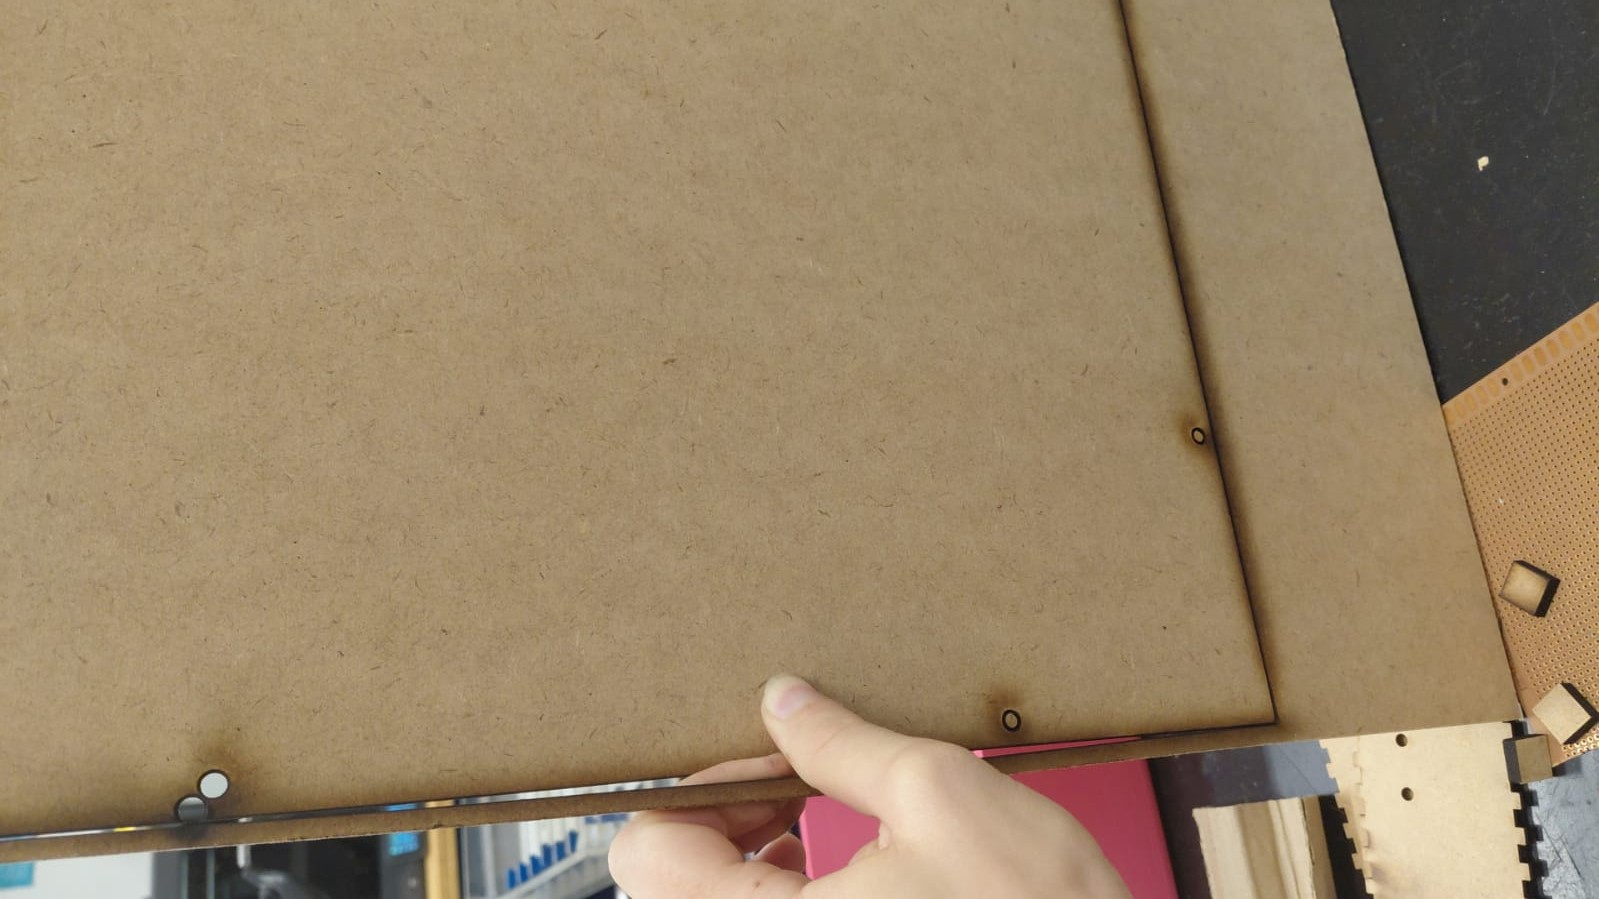
\includegraphics[width=\textwidth]{imagens/cortelaser.jpeg}
        \caption{Falhas no corte do MDF.}
    \end{subfigure}
    \hfill
    \begin{subfigure}[b]{0.45\textwidth}
        \centering
        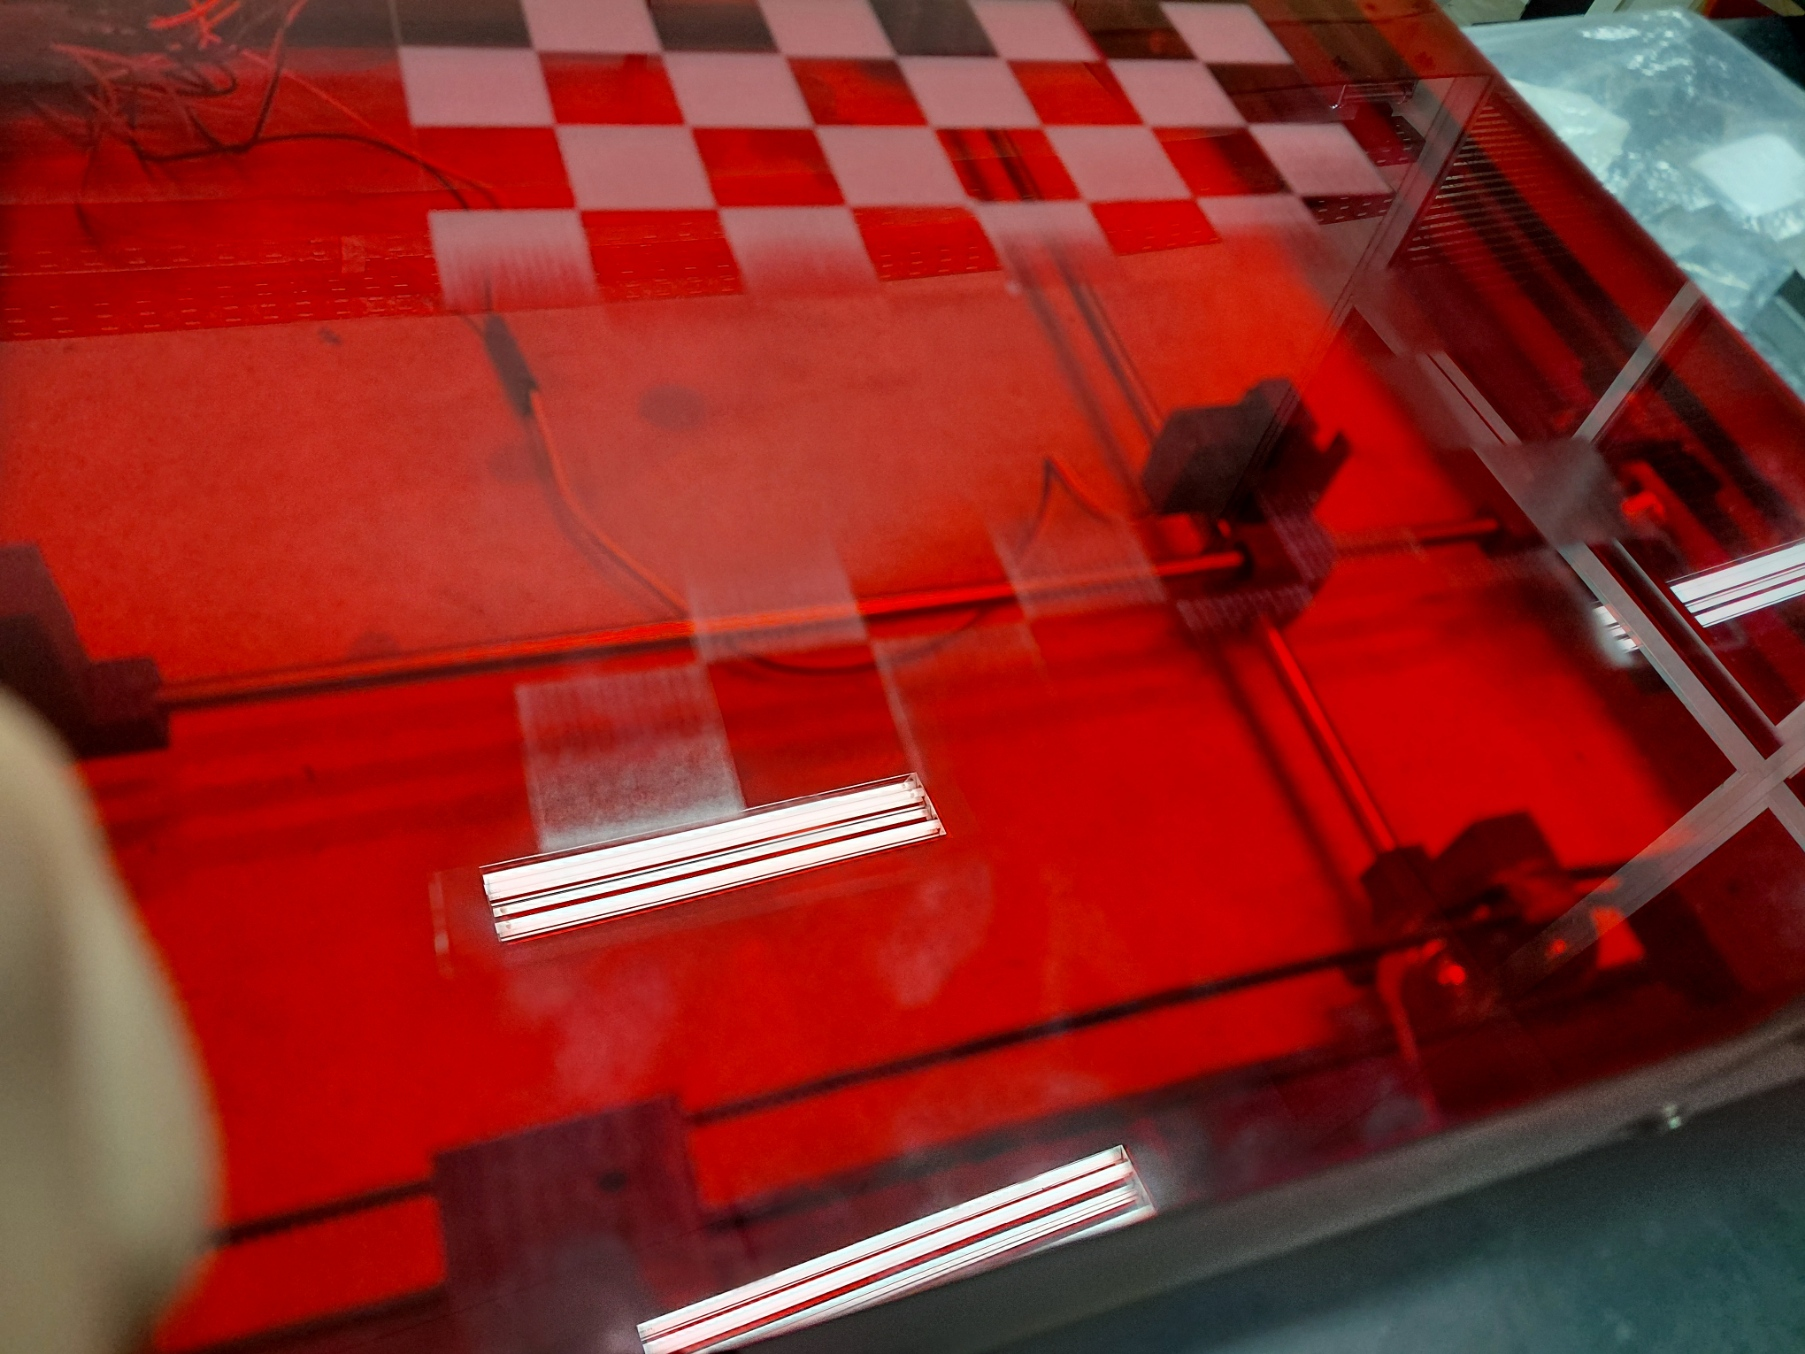
\includegraphics[width=\textwidth]{imagens/tampa1.jpg}
        \caption{Falhas no desenho do acrílico.}
    \end{subfigure}
    \caption{Problemas oriundos da perda de potência na cortadora a laser.}
    \label{fig:laser_falhas}
\end{figure}

\subsection{Mapeamento Físico e Peças do Jogo}
As peças foram desenhadas e impressas com dimensões que permitissem a passagem livre entre as demais casas ocupadas. Por serem leves demais, os campos magnéticos parasitas de componentes vizinhos provocavam atração mútua e tombamentos. Para contornar esse problema, as peças foram confeccionadas em impressão 3D contendo uma cavidade cilíndrica interna projetada para abrigar um parafuso de aço Allen M6. A cabeça sextavada do parafuso forneceu o diâmetro e a profundidade ideais para embutir um pequeno ímã de neodímio de $4\,\text{mm} \times 2\,\text{mm}$ (Figura \ref{fig:pecas}). O peso do parafuso metálico aumentou a inércia gravitacional das peças, neutralizando as forças de atração lateral e conferindo estabilidade tátil durante o movimento, além de agregar uma identidade estética agradável ao conjunto.

\begin{figure}[htpb]
    \centering
    \begin{subfigure}[b]{0.45\textwidth}
        \centering
        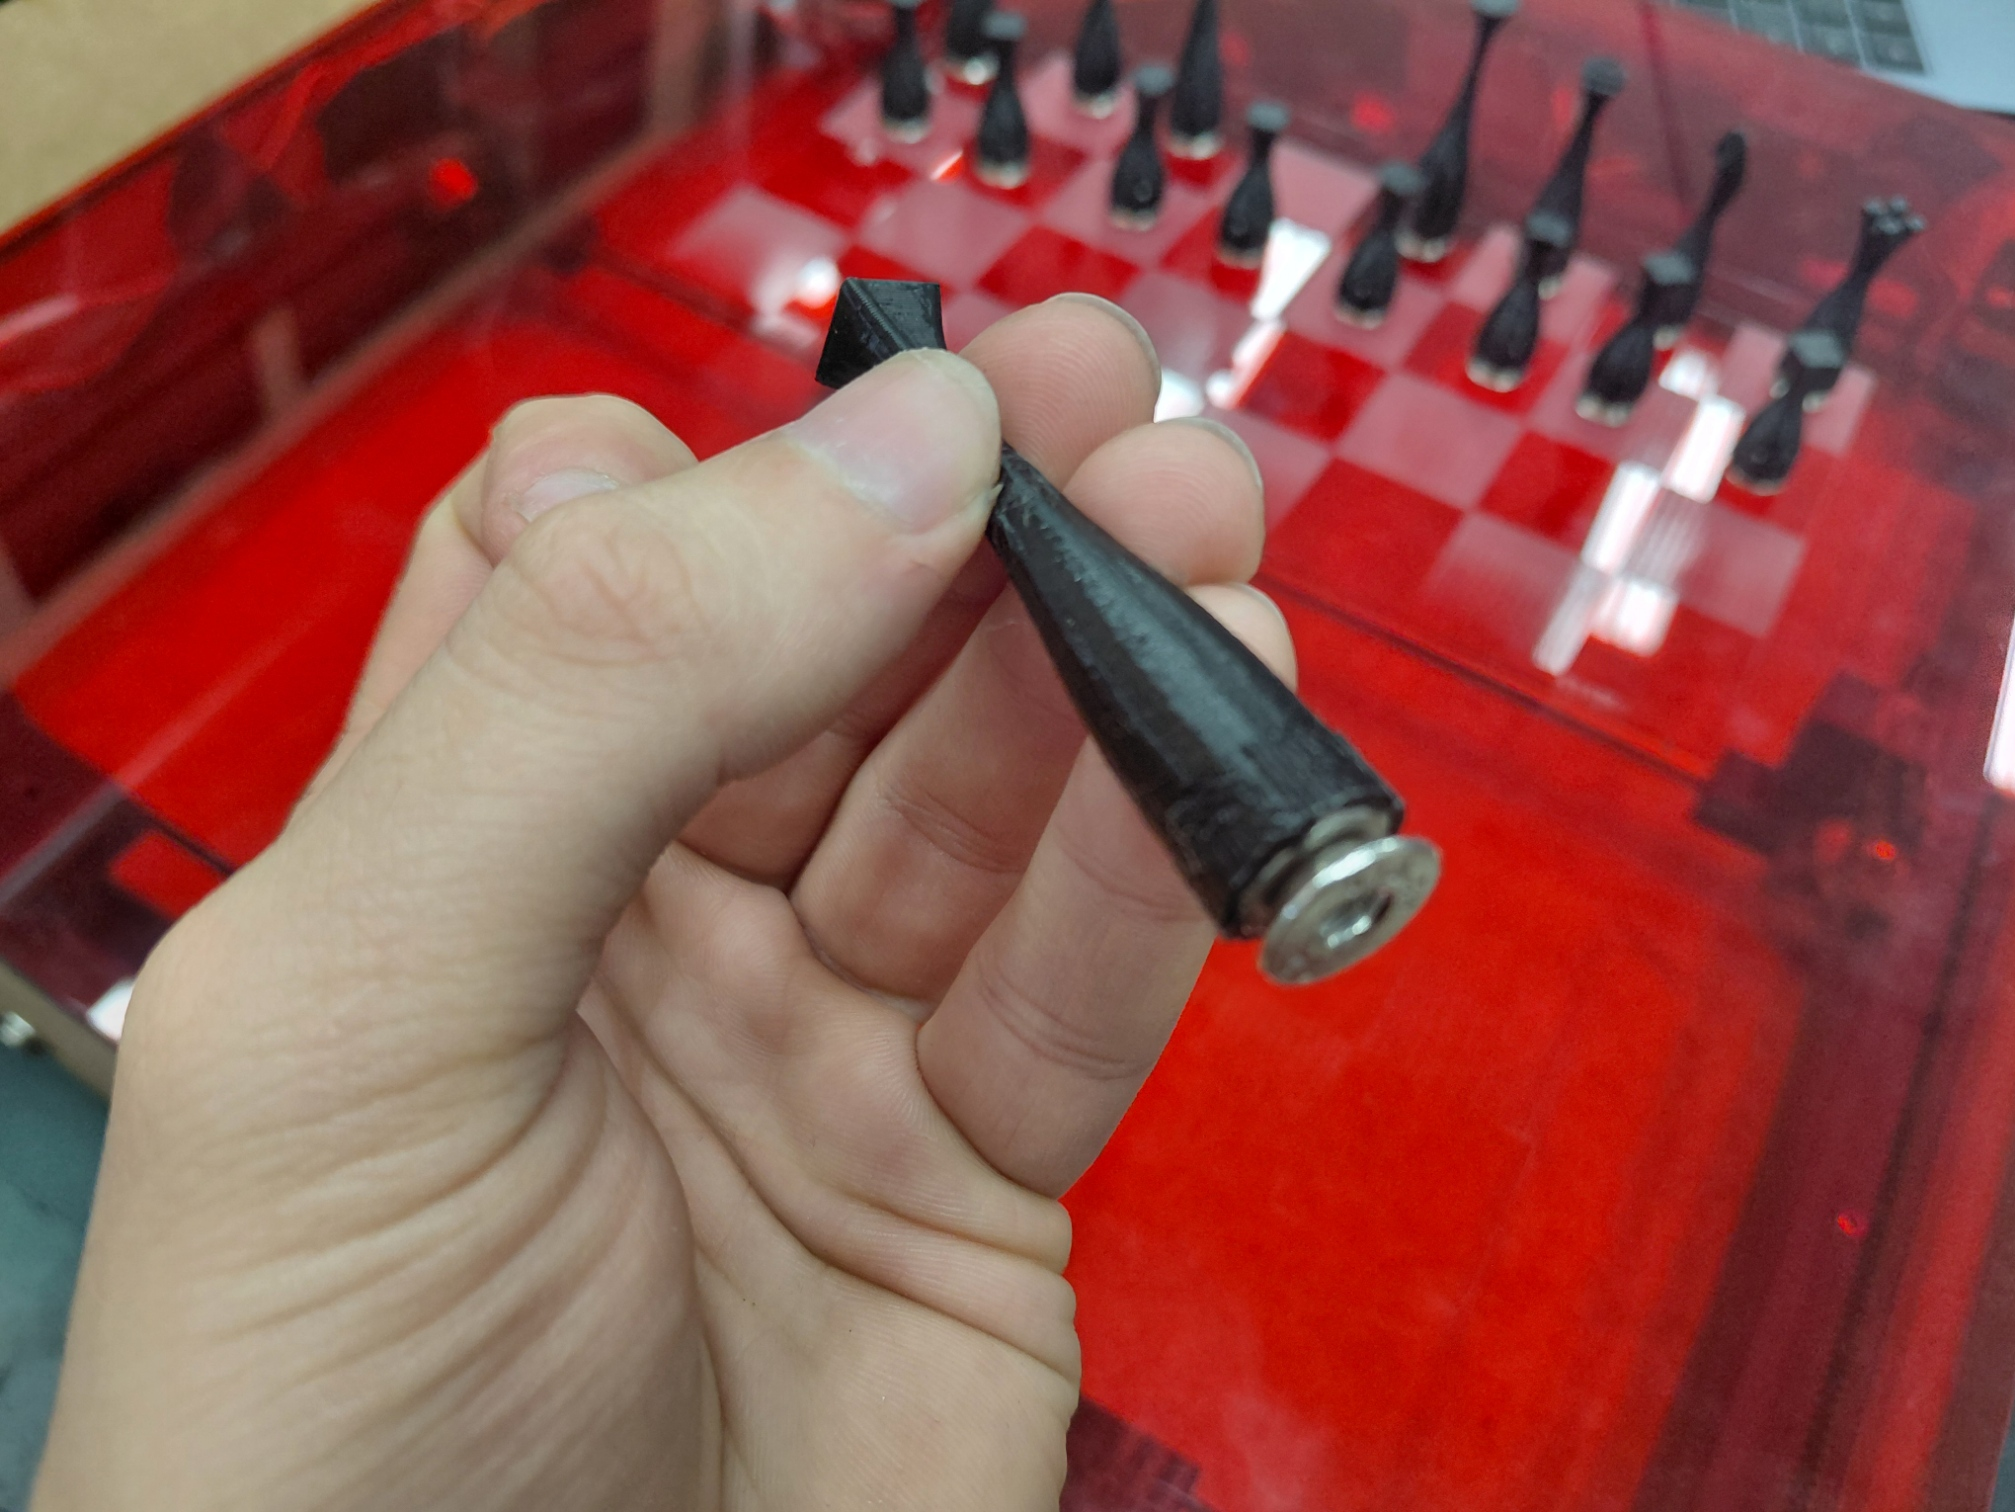
\includegraphics[width=\textwidth]{imagens/peca1.jpg}
        \caption{Peça impressa.}
    \end{subfigure}
    \hfill
    \begin{subfigure}[b]{0.45\textwidth}
        \centering
        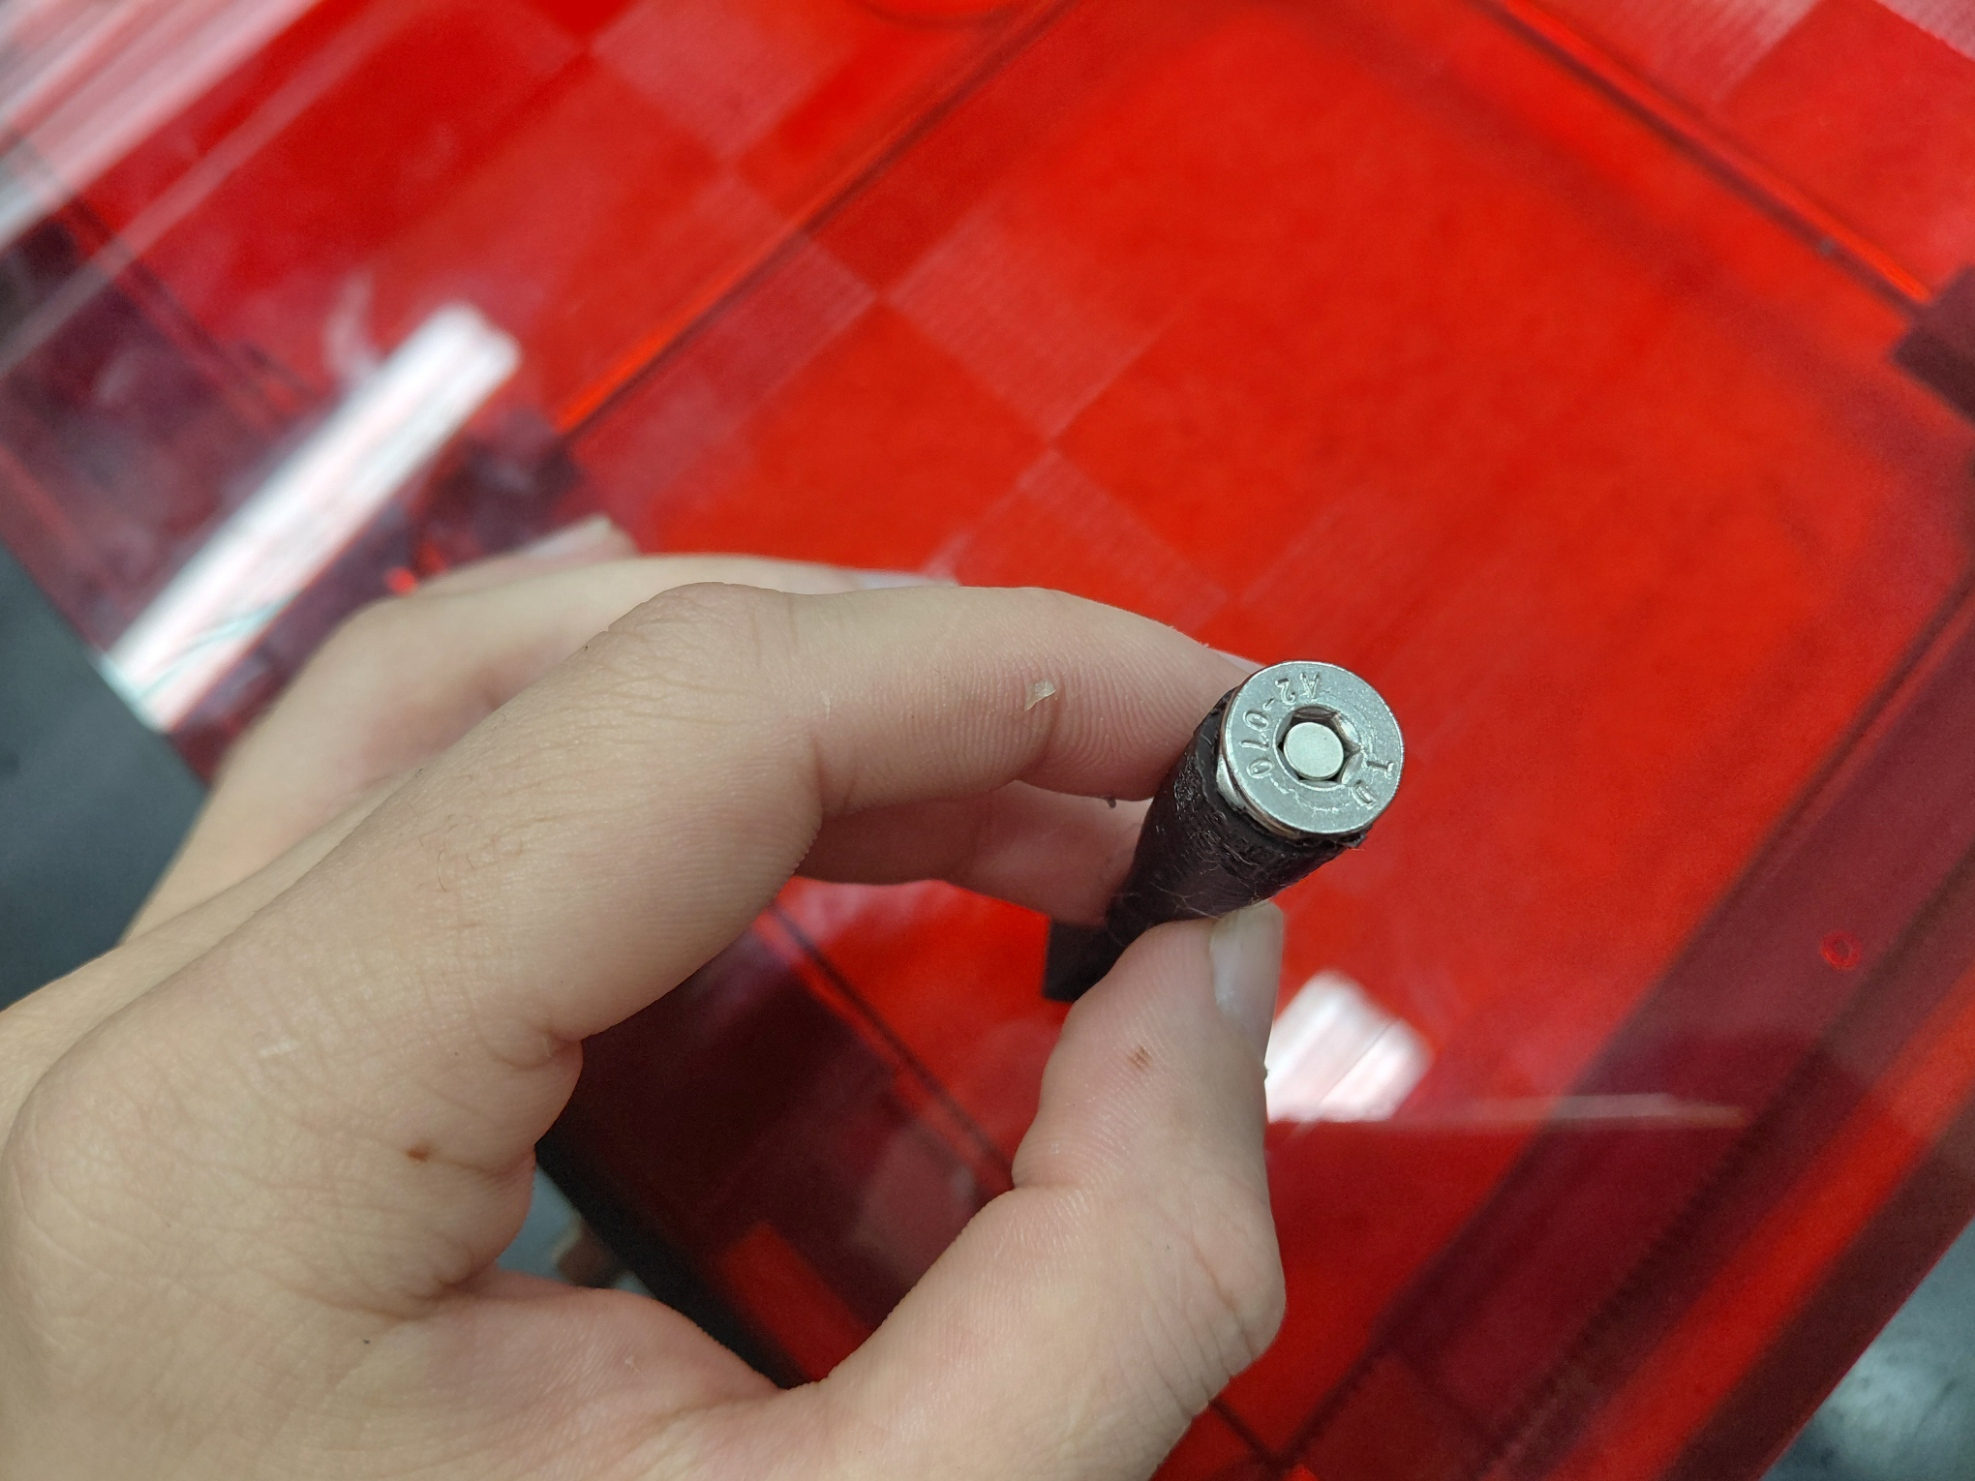
\includegraphics[width=\textwidth]{imagens/pecaima.jpg}
        \caption{Parafuso e ímã embutidos.}
    \end{subfigure}
    \caption{Adequação do peso e campo magnético das peças do tabuleiro.}
    \label{fig:pecas}
\end{figure}

Devido ao espaço interno reduzido ocupado por jumpers não planejados e às limitações geométricas impostas pelas junções coladas dos trilhos, o curso livre do carrinho ficou restrito. Originalmente planejado para casas de $3 \times 3\,\text{cm}$, as dimensões úteis foram reduzidas e a matriz de jogo de 8x8 casas foi deslocada de forma assimétrica em direção ao canto inferior direito do tabuleiro (Figura \ref{fig:tampa}). Como consequência direta dessa restrição de hardware, o sistema foi finalizado como uma prova de conceito parcial: a movimentação de jogo e as capturas no lado das brancas funcionam perfeitamente, contudo, a área de descarte lateral esquerdo das peças pretas capturadas ficou localizada além do limite físico alcançável pelo atuador cartesiano, inviabilizando partidas completas.

\begin{figure}[htpb]
    \centering
    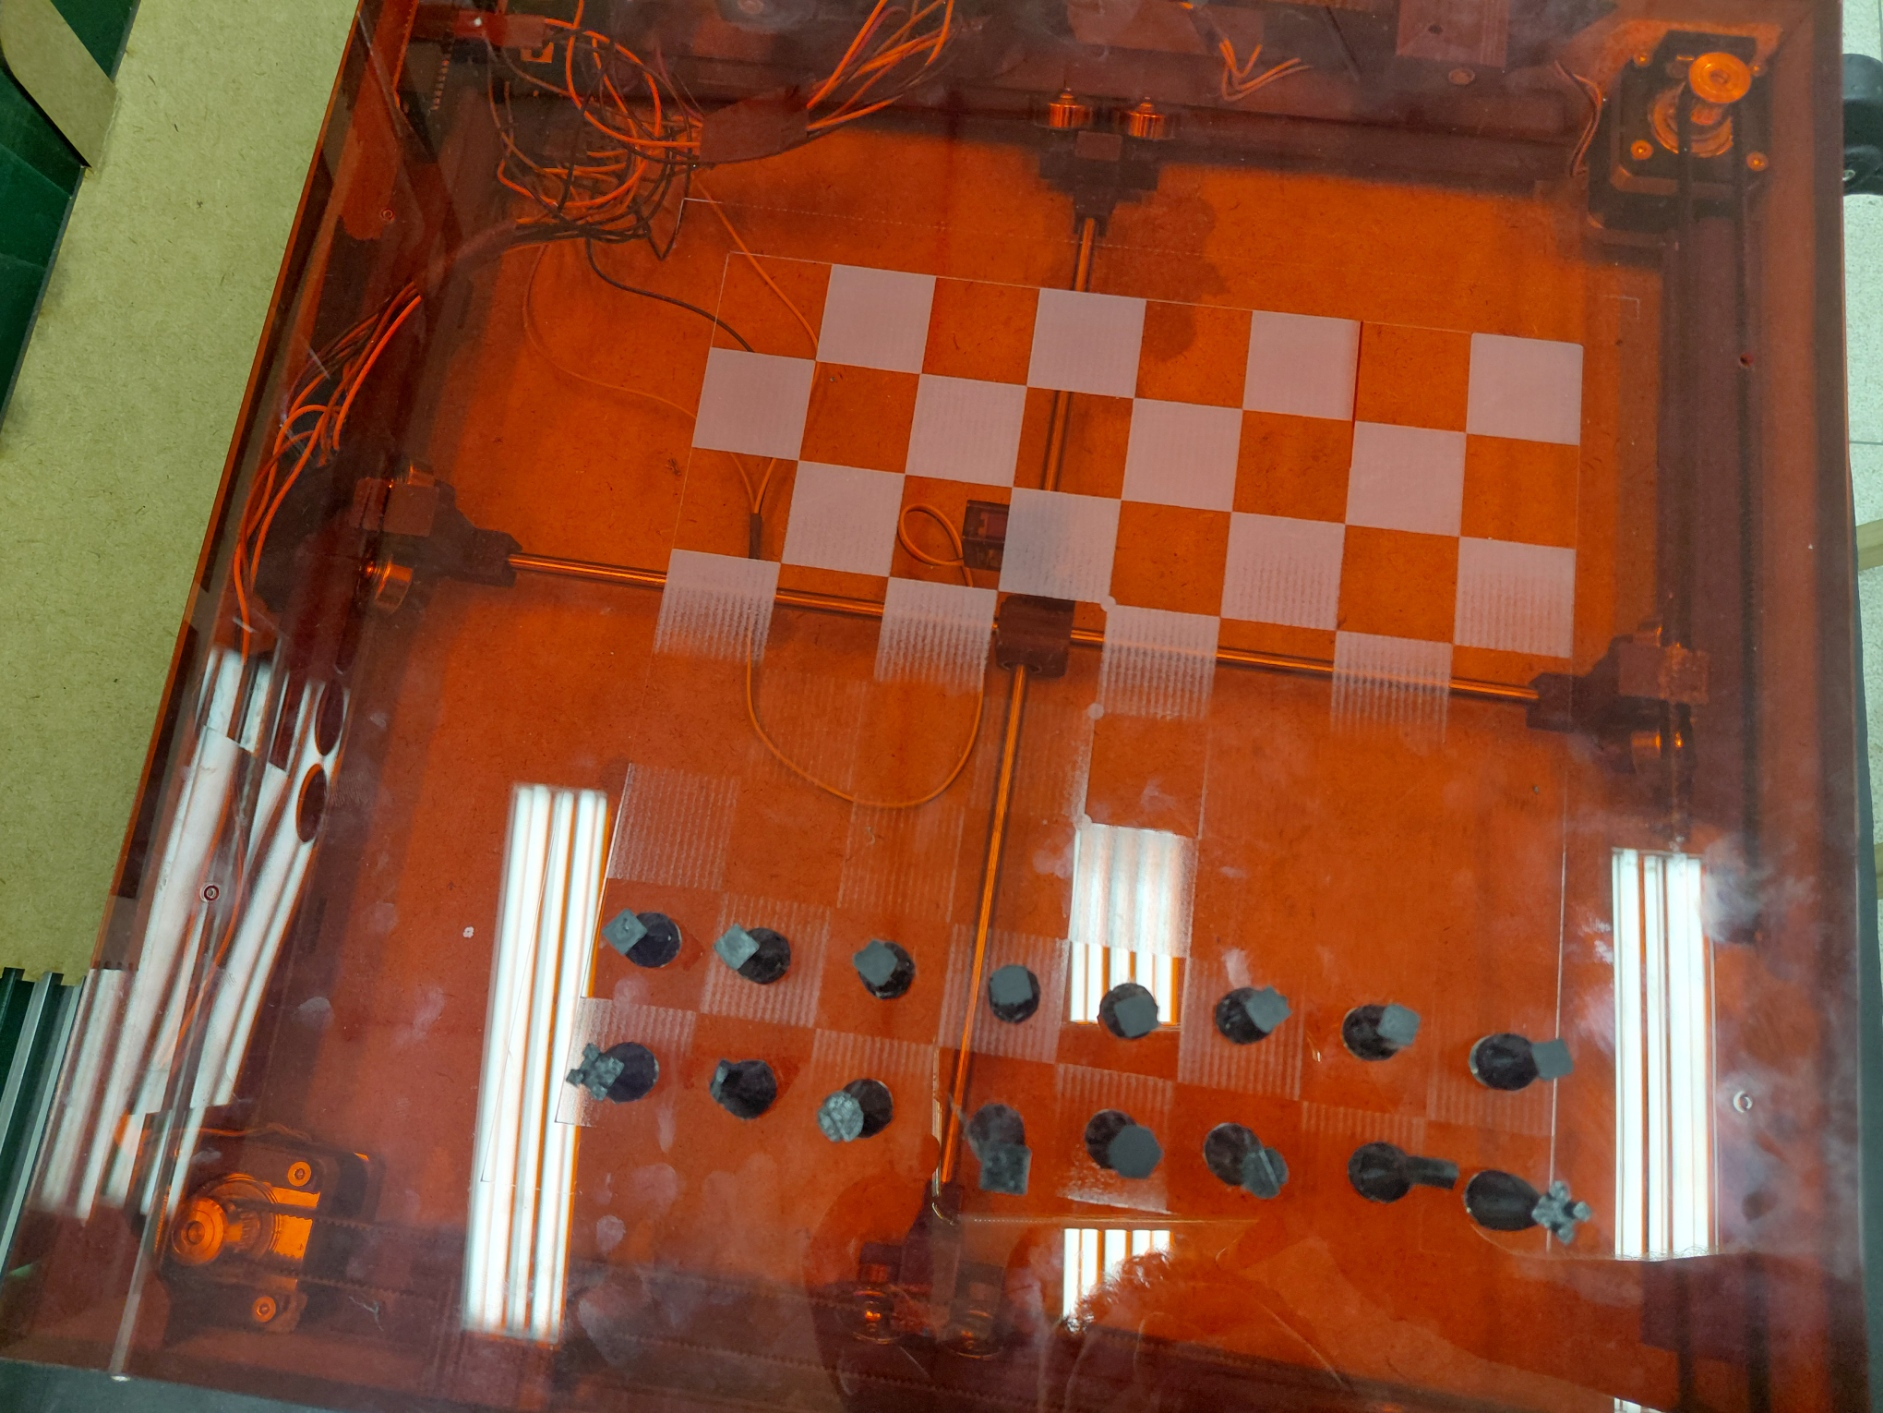
\includegraphics[width=0.7\textwidth]{imagens/tampa.jpg}
    \caption{Visão ortogonal evidenciando o deslocamento da matriz de jogo para o canto e os fios alocados internamente.}
    \label{fig:tampa}
\end{figure}

\section{Características do Protótipo e Resultados}
Dado que o projeto em si constitui o resultado prático avaliado, descrevem-se a seguir as especificações técnicas consolidadas do protótipo construído:

\begin{itemize}
    \item \textbf{Área Total:} Estrutura externa em MDF de $400 \times 400 \times 73\,\text{mm}$. Superfície superior composta por uma chapa de acrílico translúcido de 3mm, permitindo a visualização interna dos eixos em operação.
    \item \textbf{Calibração Inicial:} A calibração é feita manualmente através do comando serial \texttt{C}, que permite enviar instruções de movimentação para cada eixo individualmente. A tampa do tabuleiro possui três marcações, sendo uma central para referência de origem (\textit{Home}) (Figura \ref{fig:calibracao}). A utilização das três marcações permite a definição exata do número de passos por casa do tabuleiro.
    \item \textbf{Resolução de Movimento:} Controlado por motores NEMA 17 (1.8° por passo) operando sob subpassos eletrônicos de $1/8$ via pinos de \textit{microstepping} configurados em nível lógico alto (\lstinline{HIGH}) nos drivers A4988. A calibração prática determinou a constante de transferência de 1100 passos por casa do tabuleiro. Como cada casa é dividida em 4 elementos $a_{ij}$ da matriz interna, as coordenadas passadas para o Arduino são multiplicadas por \lstinline{STEPS_PER_SQUARE = 275}. A precisão teórica do movimento das peças é micrométrica devido ao \textit{microstepping} dos motores (1600 passos por volta), mas as folgas mecânicas nos trilhos e na cremalheira (Figura \ref{fig:gap}) limitam a precisão prática do sistema a alguns milímetros. 
    \item \textbf{Controle da Cinemática:} Operação em malha aberta estabilizada com velocidade máxima de translação parametrizada em $5000\,\text{Hz}$ (frequência de pulsos) e aceleração de $10000\,\text{Hz/s}^2$ através do algoritmo de rampa trapezoidal da biblioteca \texttt{FastAccelStepper}. Quando ocorrem trajetórias diagonais ou combinadas, o firmware calcula dinamicamente uma redução proporcional de velocidade no eixo de menor deslocamento espacial ($\Delta X$ ou $\Delta Y$), viabilizando deslocamentos diagonais síncronos.
    \begin{equation}
        \text{Se } \Delta X > \Delta Y \implies v_Y = v_{\text{max}} \cdot \left(\frac{\Delta Y}{\Delta X}\right), \quad a_Y = a_{\text{max}} \cdot \left(\frac{\Delta Y}{\Delta X}\right)
    \end{equation}
    \item \textbf{Desempenho do Software:} O processamento de voz via Whisper local em CPU atinge tempo de resposta médio de $1.2$ segundos por comando de voz. A integração com o Stockfish permite o cálculo imediato de respostas táticas com profundidade de busca limitada a 10 níveis (\textit{depth 10}), garantindo que o tempo computacional total entre a fala do usuário e o início da translação física do motor não exceda $2.5$ segundos.
\end{itemize}

\begin{figure}[htpb]
    \centering
    \begin{subfigure}[b]{0.45\textwidth}
        \centering
        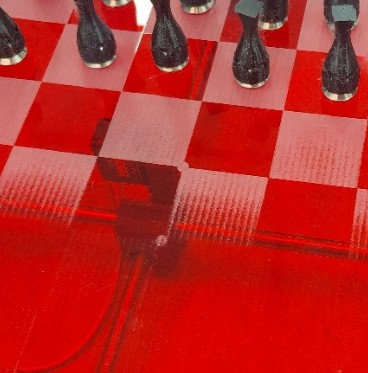
\includegraphics[width=\textwidth]{imagens/calibracao.jpg}
        \caption{Marcação central para calibração.}
        \label{fig:calibracao}
    \end{subfigure}
    \hfill
    \begin{subfigure}[b]{0.45\textwidth}
        \centering
        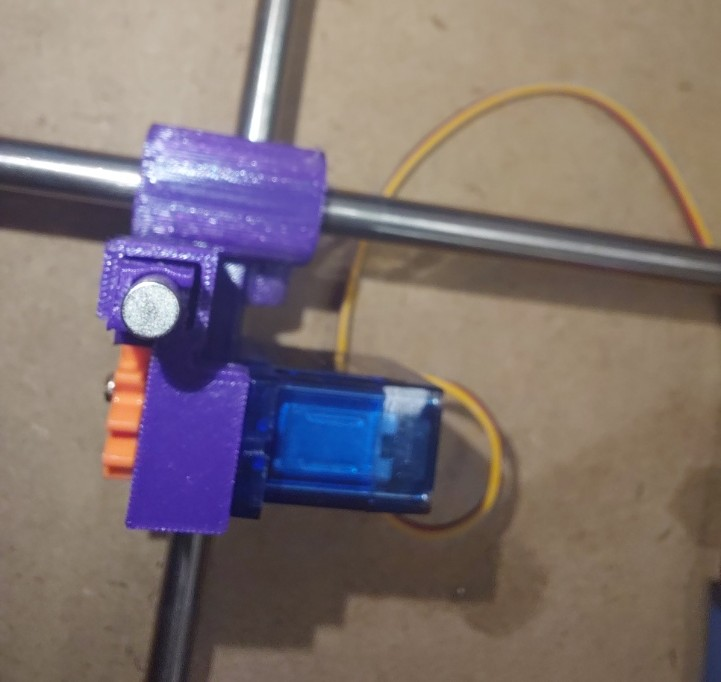
\includegraphics[width=\textwidth]{imagens/gapservo.jpg}
        \caption{Folga mecânica (gap) do atuador.}
        \label{fig:gap}
    \end{subfigure}
    \caption{Detalhes de calibração e resolução na superfície e atuador.}
    \label{fig:calibracao_gap}
\end{figure}

\section{Conclusão e Melhorias Futuras}
A execução do projeto foi bem-sucedida em seu propósito fundamental, resultando na montagem de uma plataforma mecatrônica complexa e funcional que valida a viabilidade de tabuleiros físicos controlados por voz local sem dependência de conexões de nuvem. As soluções de engenharia adotadas, como o algoritmo A* com custo de curva, o eixo flutuante para absorção de erros milimétricos de paralelismo e o ganho de peso das peças com parafusos Allen M6, permitiram contornar com êxito as severas restrições de precisão da fabricação digital em MDF e das junções dos trilhos impressos em 3D. O protótipo final (Figura \ref{fig:final}) consolidou-se como uma sólida prova de conceito de engenharia mecatrônica.

\begin{figure}[htpb]
    \centering
    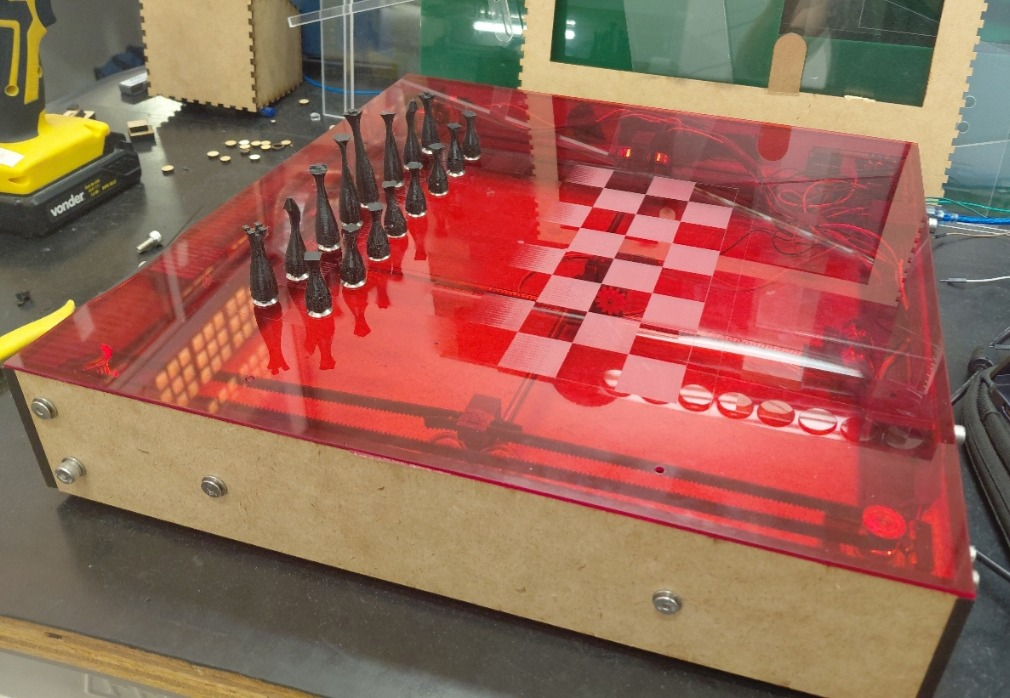
\includegraphics[width=0.8\textwidth]{imagens/final.JPG}
    \caption{Montagem final do protótipo de tabuleiro de xadrez robótico.}
    \label{fig:final}
\end{figure}

Como propostas de aperfeiçoamento para futuras versões que visem transformar o protótipo em um produto completamente funcional em toda a sua área física, destacam-se:
\begin{enumerate}
    \item Substituição integral dos trilhos e carrinhos impressos em 3D por guias lineares comerciais metálicas com patins baseados em recirculação de esferas (ex: guias MGN12), eliminando deformações por torque e folgas mecânicas;
    \item Redesenho tridimensional da carcaça interna com canais dedicados para gerenciamento de fiação e inclusão de uma placa de circuito impresso (PCB) própria, eliminando o emaranhado de jumpers flexíveis para liberar o curso total dos eixos mecânicos;
    \item Implementação de um sistema de detecção de fim de curso por chaves ópticas ou mecânicas para habilitar rotinas automáticas de calibração;
    \item Utilização de microcontroladores menores e mais potentes, como o ESP32, que possui conectividade Bluetooth integrada e estável, eliminando a necessidade de comunicação cabeada via USB; ou, alternativamente, a utilização de hardware embarcado de alto desempenho capaz de rodar os modelos locais de reconhecimento de voz e o motor de xadrez localmente, eliminando a dependência de um computador externo.
\end{enumerate}

\end{document}
